\documentclass{article}

\usepackage[english]{babel}

\usepackage[letterpaper,top=2cm,bottom=2cm,left=3cm,right=3cm,marginparwidth=1.75cm]{geometry}

% Useful packages
\usepackage{amsmath}
\usepackage{amssymb}
\usepackage{graphicx}
\usepackage{mathtools}
\usepackage{tikz}
\usepackage[colorlinks=true, allcolors=blue]{hyperref}
\usepackage{xcolor}
\usepackage{colortbl}
\usepackage{booktabs}
\usepackage{tikz}
\usepackage{tcolorbox}
\tcbuselibrary{breakable}
\usepackage{indentfirst}
\usetikzlibrary{positioning, arrows.meta}

\tcbset{
    colback=purple!5!white,
    colframe=purple!75!black,
}

\newcommand{\Fp}{\mathbb F_p}
\newcommand{\Fq}{\mathbb F_q}
\newcommand{\Pol}{T}

\title{Proximity proofs}
\author{Thomas Coratger}
\date{}
\begin{document}
\maketitle


\section{An Introduction to Linear Codes}

The journey into modern coding theory began in 1948 with Claude Shannon's groundbreaking paper, "A Mathematical Theory of Communication." He established that even over a noisy channel — like the vastness of space between a satellite and Earth, or a scratched compact disc — it's possible to transmit information with remarkable reliability. The key is to strategically add redundancy to the original message before sending it. This process, called \textbf{encoding}, transforms a message into a more robust form called a \textbf{codeword}. A \textbf{linear code} is a way to do this, using the structured language of linear algebra.

\subsection{The Core Concepts}

Before we build our first code, let's establish the fundamental concepts that allow us to measure information and errors.

\subsubsection{The Alphabet, Codewords, and the Code Itself}

First, we need an alphabet. In linear codes, this isn't just a set of symbols but a rich algebraic structure called a \textbf{finite field}, denoted $\mathbb{F}_q$. This is a set with $q$ elements where we can perform addition, subtraction, multiplication, and division with well-defined rules. 

\begin{tcolorbox}[title=Example: The Binary Field $\mathbb{F}_2$]
The simplest alphabet is the binary field $\mathbb{F}_2 = \{0, 1\}$, where addition and multiplication are performed modulo 2. For instance, $1+1=0$.
\end{tcolorbox}

With our alphabet, we can form strings. A \textbf{codeword} is a single vector (or string) of a fixed length, say $n$, composed of symbols from our alphabet. It represents one specific message after it has been encoded.

\begin{tcolorbox}[title=Example: A Binary Codeword]
The vector $\mathbf{c} = (1, 0, 1, 1, 0)$ is a single codeword of length $n=5$ in the space $\mathbb{F}_2^5$.
\end{tcolorbox}

Finally, the \textbf{code} is the complete collection of all possible valid codewords. Think of it as a dictionary: each codeword is a valid entry, and the code, denoted $\mathcal{C}$, is the entire dictionary. The goal of decoding is to determine which "dictionary entry" was sent.

\begin{tcolorbox}[title=Example: A Simple Code]
While $(1,0,1)$ is a single codeword, the set $\mathcal{C} = \{ (0,0,0), (1,0,1), (0,1,1), (1,1,0) \}$ is the entire code.
\end{tcolorbox}

\subsubsection{Measuring Errors: Hamming Weight and Distance}
To correct errors, we first need to quantify them. The Hamming metric provides an intuitive way to do this.

\paragraph{Hamming Weight}
The \textbf{Hamming weight} of a vector $\mathbf{u}$, denoted $w(\mathbf{u})$ or $|\mathbf{u}|_0$, is the number of its non-zero coordinates. It's a simple measure of how many positions are "active."

\begin{tcolorbox}[title=Example: Hamming Weight]
For the vector $\mathbf{u} = (0, 1, 0, 1, 1) \in \mathbb{F}_2^5$, we count the number of ones. The Hamming weight is $w(\mathbf{u}) = 3$.
\end{tcolorbox}

\paragraph{Hamming Distance}
The \textbf{Hamming distance} between two vectors $\mathbf{u}$ and $\mathbf{v}$, denoted $d(\mathbf{u}, \mathbf{v})$, is the number of positions in which their symbols differ. This is our fundamental measure of error — a distance of $t$ means $t$ symbols were flipped during transmission. For linear codes, there's a crucial link between distance and weight: the distance between two codewords is simply the weight of their difference: $d(\mathbf{u}, \mathbf{v}) = w(\mathbf{u} - \mathbf{v})$.

\begin{tcolorbox}[title=Example: Hamming Distance]
Let $\mathbf{u} = (1, \mathbf{0}, 1, \mathbf{1})$ and $\mathbf{v} = (1, \mathbf{1}, 1, \mathbf{0})$. They differ in the 2nd and 4th positions, so their Hamming distance is $d(\mathbf{u}, \mathbf{v}) = 2$.
\end{tcolorbox}

\subsubsection{Minimum Distance}
The single most important parameter determining a code's error-correction capability is its \textbf{minimum distance}, denoted $\ell$. This is the smallest Hamming distance between any pair of distinct codewords in the entire code. A large minimum distance means the codewords are well-separated, making it harder for noise to change one codeword into another.

For linear codes, this simplifies beautifully: the minimum distance of the code is equal to the minimum Hamming weight of all its \textbf{non-zero} codewords.
\[
   \ell = \min_{\mathbf{u}, \mathbf{v} \in \mathcal{C}, \mathbf{u} \ne \mathbf{v}} d(\mathbf{u}, \mathbf{v}) = \min_{\mathbf{w} \in \mathcal{C}, \mathbf{w} \ne \mathbf{0}} w(\mathbf{w})
\]
This is because if $\mathbf{u}$ and $\mathbf{v}$ are distinct codewords, their difference $\mathbf{u}-\mathbf{v}$ is also a non-zero codeword (due to the linearity of the code). So, finding the minimum separation between all pairs is the same as finding the "lightest" non-zero codeword.

\subsection{Formal Definition of a Linear Code}
With these concepts, we can state the formal definition. An $[n, k, \ell]_q$ linear code $\mathcal{C}$ is a $k$-dimensional linear subspace of the vector space $\mathbb{F}_q^n$ with minimum distance $\ell$.

\begin{itemize}
    \item $n$: The \textbf{block length}. This is the total length of each codeword.
    \item $k$: The \textbf{dimension}. This is the number of original message symbols. Since $\mathcal{C}$ is a $k$-dimensional subspace over $\mathbb{F}_q$, it contains exactly $|\mathcal{C}| = q^k$ unique codewords. The ratio $\rho = k/n$ is the \textbf{rate} of the code, measuring how much of the transmitted data is useful information.
    \item $\ell$: The \textbf{minimum distance}, which determines the error-correcting capability. A code with minimum distance $\ell$ can detect up to $\ell-1$ errors and correct up to $t = \lfloor(\ell-1)/2\rfloor$ errors.
    \item $q$: The \textbf{size of the finite field} (the alphabet).
\end{itemize}

\subsection{Constructing a Linear Code: The Generator Matrix}
Because a linear code is a vector subspace, we can describe the entire set of $q^k$ codewords using a small basis of just $k$ vectors. We arrange these basis vectors as the rows of a $k \times n$ matrix called the \textbf{generator matrix}, $G$.

This provides a simple recipe for encoding: to encode a message vector $\mathbf{m} \in \mathbb{F}_q^k$, we compute the codeword $\mathbf{c}$ via matrix multiplication:
\[
\mathbf{c} = \mathbf{m} \cdot G
\]
The full code $\mathcal{C}$ is the set of all linear combinations of the rows of $G$.

\begin{tcolorbox}[title={Example: Constructing a $[3, 2, 2]_2$ Linear Code}]

Let's build a binary code using the following $2 \times 3$ generator matrix (we will see the details later on this generator matrix, the goal here is simply to see a first full example of a linear code):
$$
G = \begin{pmatrix} 1 & 0 & 1 \\ 0 & 1 & 1 \end{pmatrix}
$$
Here, $n=3$ and $k=2$. We can generate all $2^k = 4$ codewords by multiplying each possible message vector $\mathbf{m} \in \mathbb{F}_2^2$ by $G$:

\begin{itemize}
    \item For $\mathbf{m} = (0, 0)$: $\mathbf{c} = (0,0) \cdot G = 0 \cdot (1,0,1) + 0 \cdot (0,1,1) = \mathbf{(0,0,0)}$
    \item For $\mathbf{m} = (1, 0)$: $\mathbf{c} = (1,0) \cdot G = 1 \cdot (1,0,1) + 0 \cdot (0,1,1) = \mathbf{(1,0,1)}$
    \item For $\mathbf{m} = (0, 1)$: $\mathbf{c} = (0,1) \cdot G = 0 \cdot (1,0,1) + 1 \cdot (0,1,1) = \mathbf{(0,1,1)}$
    \item For $\mathbf{m} = (1, 1)$: $\mathbf{c} = (1,1) \cdot G = 1 \cdot (1,0,1) + 1 \cdot (0,1,1) = (1+0, 0+1, 1+1) = \mathbf{(1,1,0)}$
\end{itemize}

The complete code is $\mathcal{C} = \{ (0,0,0), (1,0,1), (0,1,1), (1,1,0) \}$.

To find its minimum distance $d$, we find the weights of the non-zero codewords:
\begin{itemize}
    \item $w(1,0,1) = 2$
    \item $w(0,1,1) = 2$
    \item $w(1,1,0) = 2$
\end{itemize}
The minimum non-zero weight is 2, so $\ell=2$. This is a $[3, 2, 2]_2$ linear code. 
\end{tcolorbox}

\subsection{How Good is a Code? The Singleton Bound}

Now that we can build a code, a question arises: for a given length $n$, how much information ($k$) can we pack in while ensuring a certain error-correction capability ($\ell$)? There is a fundamental trade-off, captured by the \textbf{Singleton Bound}.

For any $[n, k, \ell]_q$ code, the parameters must satisfy:
\[
k \leq n - \ell + 1
\]
This inequality sets a hard limit on the efficiency of any code. It tells us that we cannot arbitrarily increase both the dimension $k$ (the amount of information) and the minimum distance $\ell$ (error-correction power) for a fixed block length $n$. Improving one often comes at the cost of the other.

\subsubsection{Maximum Distance Separable (MDS) Codes}

The most efficient codes are those that achieve equality in the Singleton Bound. A code is called a \textbf{Maximum Distance Separable (MDS) code} if its parameters satisfy:
\[
k = n - \ell + 1
\]
MDS codes are optimal because they offer the largest possible minimum distance for a given length and dimension, perfectly balancing information rate and error resilience.

\begin{tcolorbox}[title={Example: Checking for MDS Property}]
Let's check our $[3, 2, 2]_2$ example code against the Singleton Bound.
\begin{itemize}
    \item The parameters are $n=3$, $k=2$, and $\ell=2$.
    \item The bound states $k \leq n - \ell + 1$.
    \item Substituting the values: $2 \leq 3 - 2 + 1 \Rightarrow 2 \leq 2$.
\end{itemize}
The bound is met with equality! Our simple example code is an MDS code, meaning it's maximally efficient for its length and dimension.
\end{tcolorbox}



\subsection{The Encoding Process and Code Rate}

The generator matrix provides a simple and powerful algebraic recipe for converting any message into its corresponding protected codeword. This process is called encoding. Here, we'll detail how it works and introduce the concept of code rate, a key measure of a code's efficiency.

\subsubsection{The Encoding Map}
The process of encoding is a linear map from the $k$-dimensional space of messages to the $n$-dimensional space of codewords:
$$
\text{encode}: \mathbb{F}_q^k \to \mathbb{F}_q^n
$$
Given a message vector $\mathbf{m} = (m_1, m_2, \dots, m_k) \in \mathbb{F}_q^k$, the encoding is performed by multiplying it by the $k \times n$ generator matrix $G$:
$$
\mathbf{c} = \mathbf{m} \cdot G
$$
The resulting codeword $\mathbf{c}$ is a vector of length $n$ that now includes structured redundancy.

A particularly useful type of generator matrix is one in \textbf{standard form}, $G = [I_k | A]$, where $I_k$ is the $k \times k$ identity matrix. An encoder using such a matrix is called a \textbf{systematic encoder}, because the original message $\mathbf{m}$ appears unchanged in the first $k$ positions of the codeword $\mathbf{c}$. The remaining $n-k$ positions are the added redundancy, often called parity check symbols.

\begin{tcolorbox}[title={Example: Encoding a Single Message}]
Let's use our $[3, 2, 2]_2$ code from the previous example, which has the generator matrix:
\[
G = \begin{pmatrix} 1 & 0 & 1 \\ 0 & 1 & 1 \end{pmatrix}
\]
Suppose we want to encode the message $\mathbf{m} = (1, 1) \in \mathbb{F}_2^2$. We compute the product $\mathbf{m} \cdot G$:
\begin{align*}
\mathbf{c} &= (1, 1) \cdot \begin{pmatrix} 1 & 0 & 1 \\ 0 & 1 & 1 \end{pmatrix} \\
&= (1 \cdot 1 + 1 \cdot 0, \quad 1 \cdot 0 + 1 \cdot 1, \quad 1 \cdot 1 + 1 \cdot 1) \\
&= (1, 1, 0)
\end{align*}
The message $(1, 1)$ is successfully encoded into the codeword $(1, 1, 0) \in \mathcal{C}$. Notice that since this $G$ is not in standard form, the original message does not appear directly in the codeword.
\end{tcolorbox}

\subsubsection{Measuring Efficiency: The Code Rate}
The \textbf{rate} of a code, denoted by $\rho$ (or often $R$), measures its efficiency. It's the ratio of the message length to the codeword length:
\[
\rho = \frac{k}{n}
\]
The rate is a value between 0 and 1. It tells us what fraction of each transmitted symbol is actual information versus redundancy.
\begin{itemize}
    \item A \textbf{high rate} (e.g., $\rho = 0.9$) means the code is very efficient, with little redundancy. This allows for faster data transmission but offers less protection against errors.
    \item A \textbf{low rate} (e.g., $\rho = 0.1$) means the code is less efficient, with a lot of redundancy. This slows down data transmission but provides much stronger error correction.
\end{itemize}
The choice of rate is always a trade-off between efficiency and reliability, dictated by the noise level of the communication channel.

\begin{tcolorbox}[title={Example: Comparing Code Rates}]
Let's compare two different codes.
\begin{enumerate}
    \item A code $\mathcal{C}_1$ has parameters $[n=10, k=5]$. It encodes 5-symbol messages into 10-symbol codewords. Its rate is:
    \[ \rho_1 = \frac{k}{n} = \frac{5}{10} = 0.5 \]
    Exactly half of the transmitted data is information, and half is redundancy.

    \item The famous $[23, 12, 7]_2$ Golay code, $\mathcal{C}_2$, encodes 12-bit messages into 23-bit codewords. Its rate is:
    \[ \rho_2 = \frac{k}{n} = \frac{12}{23} \approx 0.52 \]
    This code is slightly more efficient than $\mathcal{C}_1$ and is renowned for its powerful error-correcting capabilities, making it a classic example of a well-balanced code.
\end{enumerate}
\end{tcolorbox}

%%%%%%%%%%%%%%%%%%%%%%%%%%%%%%%%%%%%%%%%%%%%%%%%%%%%%%%
%%%%%%%%%%%%%%%%%%%%%%%%%%%%%%%%%%%%%%%%%%%%%%%%%%%%%%%
%%%%%%%%%%%%%%%%%%%%%%%%%%%%%%%%%%%%%%%%%%%%%%%%%%%%%%%

\subsection{The Unique Decoding Regime}

Now that we can construct and evaluate codes, we arrive at the central question of decoding: if we receive a corrupted vector $\mathbf{y}$, when can we determine the original codeword $\mathbf{c}$ with absolute certainty? This is the domain of \textbf{unique decoding}.

The key insight is that the minimum distance $\ell$ creates a "safe zone" or protective bubble around each codeword. As long as the number of errors is small enough that the received vector $\mathbf{y}$ remains inside the original codeword's bubble, we can reverse the damage unambiguously.

\subsubsection{The Unique Decoding Radius}
Because the minimum distance between any two distinct codewords is $\ell$, their protective bubbles can have a radius of up to (but not including) $\ell/2$ before they risk touching or overlapping. This critical value defines the code's error-correction limit.

The maximum number of errors that a code is guaranteed to correct is denoted by $t$. It is defined as:
\[
t = \left\lfloor \frac{\ell - 1}{2} \right\rfloor
\]
Any received vector with $t$ or fewer errors will always be closer to the original codeword than to any other. This value $t$ is often called the \textbf{packing radius} or the \textbf{unique decoding radius} of the code.



\begin{figure}[h!]
\centering
\tikzset{every picture/.style={line width=0.75pt}} %set default line width to 0.75pt        

\resizebox{0.80\textwidth}{!}{
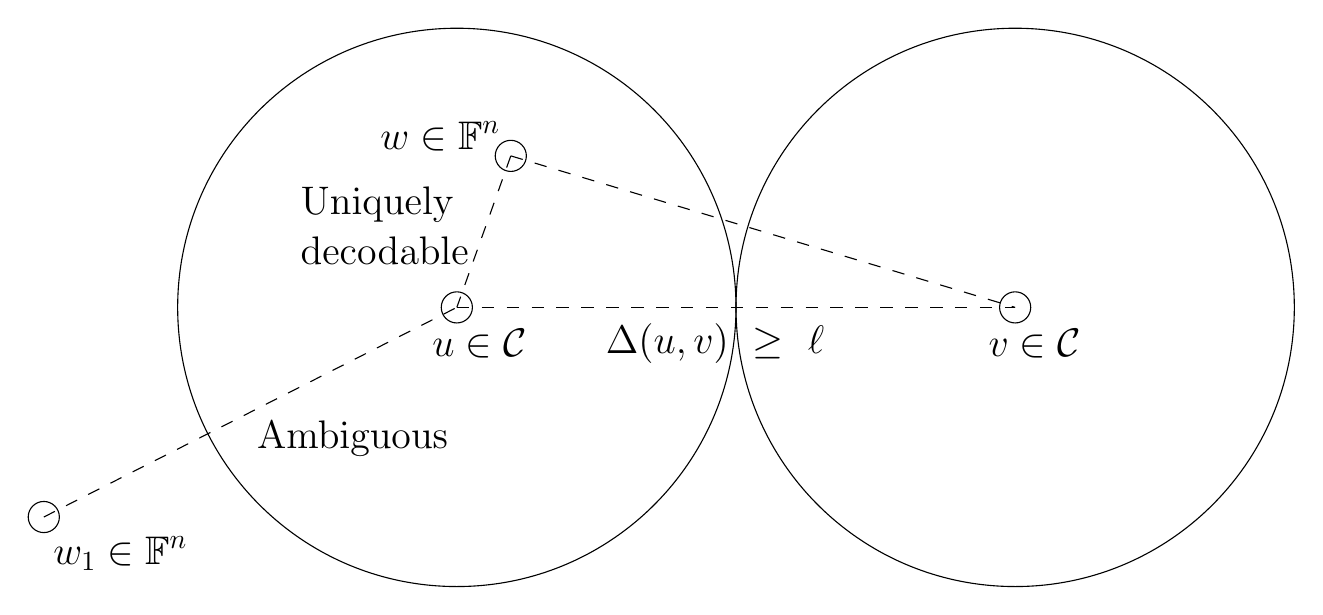
\begin{tikzpicture}[x=0.75pt,y=0.75pt,yscale=-1,xscale=1,
                    every node/.style={font=\Large}]
%uncomment if require: \path (0,300); %set diagram left start at 0, and has height of 300

%Shape: Circle [id:dp7842123195923754] 
\draw   (82,162.5) .. controls (82,88.22) and (142.22,28) .. (216.5,28) .. controls (290.78,28) and (351,88.22) .. (351,162.5) .. controls (351,236.78) and (290.78,297) .. (216.5,297) .. controls (142.22,297) and (82,236.78) .. (82,162.5) -- cycle ;
%Shape: Circle [id:dp5366130057572317] 
\draw   (351,162.5) .. controls (351,88.22) and (411.22,28) .. (485.5,28) .. controls (559.78,28) and (620,88.22) .. (620,162.5) .. controls (620,236.78) and (559.78,297) .. (485.5,297) .. controls (411.22,297) and (351,236.78) .. (351,162.5) -- cycle ;
%Shape: Circle [id:dp7225779913419981] 
\draw   (209,162.5) .. controls (209,158.36) and (212.36,155) .. (216.5,155) .. controls (220.64,155) and (224,158.36) .. (224,162.5) .. controls (224,166.64) and (220.64,170) .. (216.5,170) .. controls (212.36,170) and (209,166.64) .. (209,162.5) -- cycle ;
%Shape: Circle [id:dp20210000952005003] 
\draw   (478,162.5) .. controls (478,158.36) and (481.36,155) .. (485.5,155) .. controls (489.64,155) and (493,158.36) .. (493,162.5) .. controls (493,166.64) and (489.64,170) .. (485.5,170) .. controls (481.36,170) and (478,166.64) .. (478,162.5) -- cycle ;
%Shape: Circle [id:dp3551239038278893] 
\draw   (235,89.5) .. controls (235,85.36) and (238.36,82) .. (242.5,82) .. controls (246.64,82) and (250,85.36) .. (250,89.5) .. controls (250,93.64) and (246.64,97) .. (242.5,97) .. controls (238.36,97) and (235,93.64) .. (235,89.5) -- cycle ;
%Straight Lines [id:da49225696262016005] 
\draw  [dash pattern={on 4.5pt off 4.5pt}]  (242.5,89.5) -- (216.5,162.5) ;
%Straight Lines [id:da7593226684157609] 
\draw  [dash pattern={on 4.5pt off 4.5pt}]  (242.5,89.5) -- (485.5,162.5) ;
%Straight Lines [id:da766456784218659] 
\draw  [dash pattern={on 4.5pt off 4.5pt}]  (216.5,162.5) -- (485.5,162.5) ;
%Shape: Circle [id:dp3149209639848256] 
\draw   (10,263.5) .. controls (10,259.36) and (13.36,256) .. (17.5,256) .. controls (21.64,256) and (25,259.36) .. (25,263.5) .. controls (25,267.64) and (21.64,271) .. (17.5,271) .. controls (13.36,271) and (10,267.64) .. (10,263.5) -- cycle ;
%Straight Lines [id:da7884429019568807] 
\draw  [dash pattern={on 4.5pt off 4.5pt}]  (17.5,263.5) -- (216.5,162.5) ;

% Text Node
\draw (225,80) node   [align=left] {\begin{minipage}[lt]{68pt}\setlength\topsep{0pt}
$\displaystyle w\in \mathbb{F}^{n} \ $
\end{minipage}};
% Text Node
\draw (250,180) node   [align=left] {\begin{minipage}[lt]{68pt}\setlength\topsep{0pt}
$\displaystyle u\in \mathcal{C} \ $
\end{minipage}};
% Text Node
\draw (518,180) node   [align=left] {\begin{minipage}[lt]{68pt}\setlength\topsep{0pt}
$\displaystyle v\in \mathcal{C} \ $
\end{minipage}};
% Text Node
\draw (355,180) node   [align=left] {\begin{minipage}[lt]{100pt}\setlength\topsep{0pt}
$\displaystyle \Delta ( u,v) \ \geq \ \ell $
\end{minipage}};
% Text Node
\draw (140,103) node [anchor=north west][inner sep=0.75pt]   [align=left] {Uniquely \\decodable};
% Text Node
\draw (119,216) node [anchor=north west][inner sep=0.75pt]   [align=left] {Ambiguous};
% Text Node
\draw (67.5,281) node   [align=left] {\begin{minipage}[lt]{68pt}\setlength\topsep{0pt}
$\displaystyle w_{1} \in \mathbb{F}^{n} \ $
\end{minipage}};

\end{tikzpicture}}
\caption{The unique decoding radius creates non-overlapping "safe zones" around codewords. A received $w \in \mathbb{F}^n$ inside a zone is uniquely decodable, while $w_1 \in \mathbb{F}^n$ outside is ambiguous.}
\label{fig:decoding_bubbles}
\end{figure}





\paragraph{The Uniqueness Guarantee}
Why can a received word only be "very close" to one codeword at most? The guarantee comes from a proof by contradiction that uses the triangle inequality.

Let's imagine for a moment that a received word $\mathbf{w}$ \textit{is} very close to two different codewords, $\mathbf{u}$ and $\mathbf{v}$. To be "very close" means the distance is less than half the minimum separation, $\ell/2$. So we assume:
\begin{itemize}
    \item The number of errors between $\mathbf{w}$ and $\mathbf{u}$ is small: $d(\mathbf{w}, \mathbf{u}) < \ell/2$.
    \item The number of errors between $\mathbf{w}$ and $\mathbf{v}$ is also small: $d(\mathbf{w}, \mathbf{v}) < \ell/2$.
\end{itemize}
The triangle inequality tells us that the direct path between two points is always the shortest. Going from $\mathbf{u}$ to $\mathbf{v}$ via the "detour" of $\mathbf{w}$ cannot be shorter:
\[
\underbrace{d(\mathbf{u}, \mathbf{v})}_{\text{Direct distance}} \leq \underbrace{d(\mathbf{u}, \mathbf{w})}_{\text{Detour part 1}} + \underbrace{d(\mathbf{w}, \mathbf{v})}_{\text{Detour part 2}}
\]
Now, let's see what our assumption implies. Since each part of the detour is shorter than $\ell/2$, their sum must be less than $\ell$:
\[
d(\mathbf{u}, \mathbf{v}) < \underbrace{\frac{\ell}{2}}_{\text{An upper bound for } d(\mathbf{u},\mathbf{w})} + \underbrace{\frac{\ell}{2}}_{\text{An upper bound for } d(\mathbf{v},\mathbf{w})} = \ell
\]
This conclusion, $d(\mathbf{u}, \mathbf{v}) < \ell$, says that the distance between codewords $\mathbf{u}$ and $\mathbf{v}$ is less than the \textit{minimum possible distance} $\ell$. This is a logical impossibility.

Therefore, our initial assumption was wrong. A received word $\mathbf{w}$ cannot be simultaneously "very close" (unique decoding regime) to two different codewords.

\begin{tcolorbox}[title={Example: Unique Decoding in Action}]
\paragraph{Case 1: An Ambiguous Code ($t=0$)}
Let's first revisit our $[3, 2, 2]_2$ code.
\begin{itemize}
    \item Parameters: $n=3$, $k=2$, $\ell=2$.
    \item The code is $\mathcal{C} = \{ (0,0,0), (1,0,1), (0,1,1), (1,1,0) \}$.
    \item Unique decoding radius: $t = \lfloor (\ell-1)/2 \rfloor = \lfloor (2-1)/2 \rfloor = 0$.
\end{itemize}
A radius of $t=0$ means this code can \textbf{guarantee to correct 0 errors}. It can detect 1 error, but cannot reliably correct it. Suppose the received vector is $\mathbf{w} = (1,0,0)$. The number of errors is 1, which is greater than $t$. As expected, decoding is ambiguous:
\begin{itemize}
    \item $d(\mathbf{w}, (0,0,0)) = 1$
    \item $d(\mathbf{w}, (1,0,1)) = 1$
    \item $d(\mathbf{w}, (1,1,0)) = 1$
\end{itemize}
The received vector $\mathbf{w}$ is equally close to three different codewords, so the decoder fails.

\hrulefill

\paragraph{Case 2: A Uniquely Decodable Code ($t=1$)}
Now, let's consider a code designed for error correction: the $[3, 1, 3]_2$ repetition code.
\begin{itemize}
    \item Parameters: $n=3$, $k=1$, $\ell=3$.
    \item The code is $\mathcal{C} = \{ (0,0,0), (1,1,1) \}$.
    \item Unique decoding radius: $t = \lfloor (3-1)/2 \rfloor = 1$.
\end{itemize}
A radius of $t=1$ means this code is \textbf{guaranteed to correct any single-bit error}.

Suppose we send $\mathbf{c} = (1,1,1)$ and a single error occurs, flipping the first bit. The received vector is $\mathbf{w} = (0,1,1)$. The number of errors is 1, which is within our decoding radius ($1 \le t$). Let's find the closest codeword to $\mathbf{w}$:
\begin{itemize}
    \item $d(\mathbf{w}, (0,0,0)) = w(0,1,1) = 2$
    \item $d(\mathbf{w}, (1,1,1)) = w(1,0,0) = 1$
\end{itemize}
The received vector $\mathbf{w}$ is uniquely closest to $(1,1,1)$. The decoder correctly identifies the original codeword, successfully correcting the error.
\end{tcolorbox}


%%%%%%%%%%%%%%%%%%%%%%%%%%%%%%%%%%%%%%%%%%%%%%%%%%%%%%%
%%%%%%%%%%%%%%%%%%%%%%%%%%%%%%%%%%%%%%%%%%%%%%%%%%%%%%%
%%%%%%%%%%%%%%%%%%%%%%%%%%%%%%%%%%%%%%%%%%%%%%%%%%%%%%%

\subsection{Why Unique Decoding Isn't Enough}
Unique decoding provides a wonderful guarantee, but it comes with a strict limitation: it only works if the number of errors is very small. If the noise on a channel is higher, a received word $\mathbf{w}$ is highly likely to fall outside of any "safe zone." This leads to a crucial question: just how many words are actually uniquely decodable?

As we will see, the answer is a surprisingly small fraction. This limitation is the primary motivation for more advanced techniques like \textbf{list decoding}.

\paragraph{Counting the "Safe" Words}
To understand the problem, let's count how many vectors are in one of these uniquely decodable bubbles. A \textbf{Hamming ball} of radius $t$ around a codeword $\mathbf{u}$, denoted $B(\mathbf{u}, t)$, is the set of all vectors $\mathbf{w}$ that are at a distance of $t$ or less from $\mathbf{u}$.





The number of vectors in this ball is the sum of the counts for every possible number of errors, from 0 up to $t$. To understand the formula's origin, let's first figure out how to count the number of vectors with \textit{exactly} $i$ errors. This is a two-step process:
\begin{enumerate}
    \item \textbf{Choose the error positions:} First, where did the errors occur? We need to choose which $i$ of the $n$ total positions in the vector were corrupted. The number of ways to do this is given by the binomial coefficient $\binom{n}{i}$.
    \item \textbf{Choose the new symbols:} For each of the $i$ positions that have an error, the original symbol must be changed to a different one. Our alphabet is the field $\mathbb{F}_q$, which has $q$ total symbols. This means for each error, there are $(q-1)$ other symbols to choose from. Since there are $i$ errors, there are $(q-1)^i$ ways to choose the new symbols.
\end{enumerate}

Therefore, the total number of vectors with exactly $i$ errors is the product of these two parts: $\binom{n}{i} (q-1)^i$. To get the total size of the Hamming ball, we simply sum the counts for all possible numbers of errors, from $i=0$ (no errors) up to the maximum we can correct, $t$:
\[
|B(\mathbf{u}, t)| = \sum_{i=0}^{t} \underbrace{\binom{n}{i}}_{\text{Ways to choose } i \text{ error positions}} \times \underbrace{(q-1)^i}_{\text{Ways to choose new symbols for them}}
\]
This formula counts every possible vector that can be reached from $\mathbf{u}$ by introducing at most $t$ errors.

\begin{tcolorbox}[breakable, title={A Quick Refresher on the Binomial Coefficient $\binom{n}{k}$}]
The notation $\binom{n}{k}$, read as "$n$ choose $k$", represents the number of ways to select $k$ items from a set of $n$ distinct items, where the order of selection doesn't matter.


The general formula is:
\[ \binom{n}{k} = \frac{n!}{k!(n-k)!} \]
where $n!$ (n-factorial) is $n \times (n-1) \times \dots \times 1$. 
In our main formula, $\binom{n}{i}$ is simply counting all the possible ways that $i$ errors can be distributed among the $n$ positions of a codeword.
\end{tcolorbox}





\begin{tcolorbox}[title={Example: Counting Words in a Hamming Ball}]
Let's use a code over the ternary field $\mathbb{F}_3$ (so $q=3$) with block length $n=10$. Suppose its minimum distance is $\ell=7$, which gives a unique decoding radius of $t = \lfloor(7-1)/2\rfloor = 3$.

How many words are in the Hamming ball of radius 3 around a single codeword $\mathbf{u}$?
\[ |B(\mathbf{u}, 3)| = \sum_{i=0}^{3} \binom{10}{i}(3-1)^i = \binom{10}{0}2^0 + \binom{10}{1}2^1 + \binom{10}{2}2^2 + \binom{10}{3}2^3 \]
Let's calculate term by term:
\begin{itemize}
    \item 0 errors: $\binom{10}{0} \cdot 1 = 1 \cdot 1 = 1$ (just the codeword itself)
    \item 1 error:  $\binom{10}{1} \cdot 2 = 10 \cdot 2 = 20$
    \item 2 errors: $\binom{10}{2} \cdot 4 = 45 \cdot 4 = 180$
    \item 3 errors: $\binom{10}{3} \cdot 8 = 120 \cdot 8 = 960$
\end{itemize}
The total number of words in this single decoding bubble is $1 + 20 + 180 + 960 = \mathbf{1,161}$.

Now, let's compare this to the total number of possible vectors in the entire space $\mathbb{F}_3^{10}$. There are $3^{10} = \mathbf{59,049}$ possible vectors.

So, the "safe zone" for a single codeword covers only $1,161 / 59,049 \approx 1.9\%$ of the entire space. Even if we sum this over all codewords in a high-rate code, the total uniquely decodable volume remains a tiny fraction of the whole space.
\end{tcolorbox}


The example and the demonstration above reveal something important. The set of all uniquely decodable words (the union of all Hamming balls around all codewords) is almost always \textit{exponentially smaller} than the total space of all possible received words, $\mathbb{F}_q^n$.

This means that if a received word $\mathbf{w}$ suffers from more than $t$ errors, it will land in the vast and ambiguous space between the decoding bubbles. In this scenario, asking the decoder for a single, unique answer is asking the wrong question.

This is precisely why we need \textbf{list decoding}. Instead of demanding a single answer, we relax the question to: can you give me a short list of \textit{all} codewords that are reasonably close to the received word?

This approach acknowledges that ambiguity is likely and provides a way to manage it, forming the basis for many modern and powerful decoding algorithms.



%%%%%%%%%%%%%%%%%%%%%%%%%%%%%%%%%%%%%%%%%%%%%%%%%%%%%%%
%%%%%%%%%%%%%%%%%%%%%%%%%%%%%%%%%%%%%%%%%%%%%%%%%%%%%%%
%%%%%%%%%%%%%%%%%%%%%%%%%%%%%%%%%%%%%%%%%%%%%%%%%%%%%%%


\subsection{List Decoding}

We've seen that the guarantee of unique decoding is powerful but fragile. It only applies within a small "safe zone" around each codeword. If a received word $\mathbf{w}$ suffers from more errors than the unique decoding radius $t$, it lands in the vast, ambiguous space where it might be close to several codewords at once.

Instead of giving up, we can change our goal. This leads to the idea of \textbf{list decoding}.

\subsubsection{Motivation: A More Realistic Question}
The problem with unique decoding is that it insists on a single, unambiguous answer. When that's not possible, it fails. List decoding takes a more different approach by asking a more flexible question: Instead of the \textit{one} true codeword, can you give me a short \textit{list} of all plausible candidates?

The goal is no longer to find a single answer but to efficiently produce a small list of all codewords $\mathbf{u} \in \mathcal{C}$ that are within a certain distance $e$ of the received word $\mathbf{w}$.

The immediate question, however, is: how long could this list be? If it's potentially enormous, it's not very useful. This is where a remarkable result, the Johnson bound, provides a crucial guarantee.

\subsubsection{The Johnson Bound: A Limit on Ambiguity}
The \textbf{Johnson bound} is a universal "safety net" for decoding. It tells us that even when we are outside the unique decoding radius, the number of nearby codewords doesn't immediately explode. For a significant range of errors, the list of candidates remains small and manageable.

To state the bound formally, we use the \textit{relative} parameters of the code:
\begin{itemize}
    \item The \textbf{relative minimum distance}, $\mu = \ell / n$.
    \item The \textbf{relative decoding radius} (or fraction of errors), $\delta = e / n$, where $e$ is the number of errors we want to tolerate.
\end{itemize}

\begin{tcolorbox}[breakable, title={The Johnson Bound}]
Let $\mathcal{C}$ be any code with relative minimum distance $\mu$. For any received word $\mathbf{w}$, the number of codewords within a relative distance $\delta$ is bounded, as long as $\delta$ is less than the \textbf{Johnson radius}:
\[
\delta < 1 - \sqrt{1-\mu}
\]
Inside this radius, the size of the list of candidate codewords is guaranteed to be small. Specifically, for binary codes ($q=2$), the list size is bounded by approximately $n$. For general $q$, the bound is more complex but remains polynomial in $n$.

This is a powerful result because the bound depends only on the distance parameters $\mu$ and $\delta$, not on the specific structure of the code.
\end{tcolorbox}

The Johnson bound reveals that the ambiguity of decoding grows in a controlled way. It doesn't become chaotic as soon as we leave the unique decoding radius.

\subsubsection{The Three Regimes of Decoding}
We can now summarize the entire decoding landscape based on the fraction of errors, $\delta$, we are trying to correct.

\begin{figure}[h!]
\centering
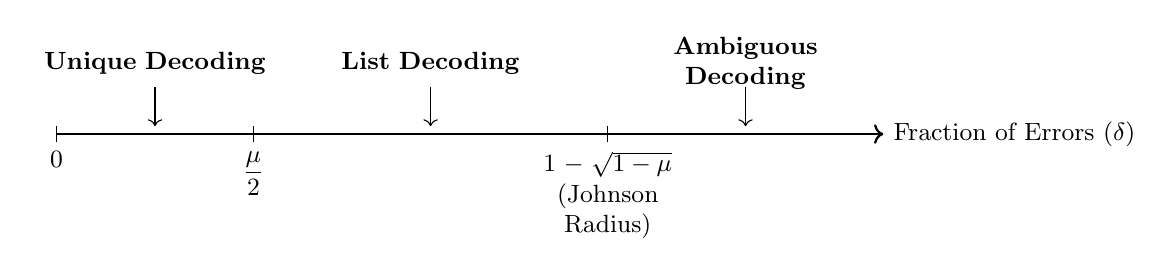
\begin{tikzpicture}[font=\small]
    % Draw the main axis
    \draw[->, thick] (0,0) -- (10.5,0) node[right] {Fraction of Errors ($\delta$)};
    
    % Mark the points
    \draw (0,0.1) -- (0,-0.1) node[below] {$0$};
    \node (ud) at (2.5,0) {};
    \draw (ud) ++(0,0.1) -- ++(0,-0.2) node[below] {$\dfrac{\mu}{2}$};
    \node (jb) at (7,0) {};
    \draw (jb) ++(0,0.1) -- ++(0,-0.2) node[below, text width=2.5cm, align=center] {$1 - \sqrt{1-\mu}$ \\ (Johnson Radius)};
    
    % Label the zones (regimes)
    \node[align=center, text width=3cm, black] at (1.25, 0.9) {\textbf{Unique Decoding}};
    \draw[->, black] (1.25, 0.6) -- (1.25, 0.1);
    
    \node[align=center, text width=3cm, black] at (4.75, 0.9) {\textbf{List Decoding}};
    \draw[->, black] (4.75, 0.6) -- (4.75, 0.1);
    
    \node[align=center, text width=3cm, black] at (8.75, 0.9) {\textbf{Ambiguous Decoding}};
    \draw[->, black] (8.75, 0.6) -- (8.75, 0.1);
\end{tikzpicture}
\caption{The three decoding regimes based on the fraction of errors $\delta$.}
\label{fig:decoding_regimes}
\end{figure}


\begin{enumerate}
    \item \textbf{Unique Decoding Regime ($\delta < \mu/2$):} This is the "safe zone" we've already discussed. The list of candidates has at most one codeword.
    \item \textbf{List Decoding Regime ($\mu/2 \leq \delta < 1-\sqrt{1-\mu}$):} Here, we can no longer guarantee a unique answer, but the Johnson bound assures us that the list of potential candidates is small. Efficient algorithms exist that can find this list.
    \item \textbf{Ambiguous Decoding Regime ($\delta \geq 1-\sqrt{1-\mu}$):} Beyond the Johnson radius, the list of candidates could be exponentially large, and decoding becomes computationally infeasible for general codes.
\end{enumerate}

The existence of the Johnson bound is crucial for modern coding theory. It proves that we can correct many more errors than the unique decoding radius suggests, as long as we are willing to accept a small list of answers instead of just one.



%%%%%%%%%%%%%%%%%%%%%%%%%%%%%%%%%%%%%%%%%%%%%%%%%%%%%%%
%%%%%%%%%%%%%%%%%%%%%%%%%%%%%%%%%%%%%%%%%%%%%%%%%%%%%%%
%%%%%%%%%%%%%%%%%%%%%%%%%%%%%%%%%%%%%%%%%%%%%%%%%%%%%%%

\subsubsection{A Note on Terminology: $\delta$-close and $\delta$-far}
To simplify our discussion of list decoding, it's helpful to have clear language to describe whether a received word is a plausible candidate for decoding or not. We use the terms \textbf{$\delta$-close} and \textbf{$\delta$-far} for this purpose.

\begin{tcolorbox}[breakable, title={Definitions}]
Let $\delta$ be a given fraction of errors (our relative decoding radius).
\begin{itemize}
    \item We say a received word $\mathbf{w}$ is \textbf{$\delta$-close} to the code $\mathcal{C}$ if there is \textit{at least one} codeword $\mathbf{u} \in \mathcal{C}$ such that $d(\mathbf{w}, \mathbf{u}) \le \delta n$. This means the list of potential candidates is not empty.

    \item We say a received word $\mathbf{w}$ is \textbf{$\delta$-far} from the code $\mathcal{C}$ if \textit{every} codeword $\mathbf{u} \in \mathcal{C}$ has a distance greater than $\delta n$ from it, i.e., $d(\mathbf{w}, \mathbf{u}) > \delta n$. In this case, the list of candidates is empty, and a list decoder would return nothing.
\end{itemize}
\end{tcolorbox}

This terminology provides a clean shorthand for discussing decoding problems. Instead of describing the conditions every time, we can simply ask: "Is the received word $\mathbf{w}$ $\delta$-close to our code?" This captures the essential geometric question of whether $\mathbf{w}$ lies within the decoding radius of any codeword in $\mathcal{C}$.


%%%%%%%%%%%%%%%%%%%%%%%%%%%%%%%%%%%%%%%%%%%%%%%%%%%%%%%
%%%%%%%%%%%%%%%%%%%%%%%%%%%%%%%%%%%%%%%%%%%%%%%%%%%%%%%
%%%%%%%%%%%%%%%%%%%%%%%%%%%%%%%%%%%%%%%%%%%%%%%%%%%%%%%

\section{Reed-Solomon Codes: Correcting Errors with Polynomials}

Having established the fundamentals of linear codes, we now turn to one of the most powerful and widely used families of error-correcting codes in history: \textbf{Reed-Solomon (RS) codes}. Invented in 1960 by Irving S. Reed and Gustave Solomon, these codes are at the heart of technologies we use every day, from storing data on CDs and Blu-ray discs to ensuring the integrity of QR codes and transmitting data from deep space probes.

The genius of Reed-Solomon codes lies in a beautifully simple idea: \textbf{representing messages as polynomials}. By leveraging the unique properties of polynomials, we can add redundancy in a highly structured way, allowing us to correct not just single-bit flips, but entire chunks of corrupted data.

\subsection{The Polynomial Toolkit}
To understand RS codes, we first need to be comfortable with the tool they are built from: polynomials.

\subsubsection{What is a Polynomial?}
A polynomial is a mathematical expression consisting of variables and coefficients. For our purposes, a message polynomial $P(x)$ is a function of a variable $x$ defined as:
\[
P(x) = m_0 + m_1 x + m_2 x^2 + \dots + m_{k-1} x^{k-1}
\]
The values $m_0, m_1, \dots, m_{k-1}$ are the \textbf{coefficients}, and the highest power of $x$ with a non-zero coefficient is the \textbf{degree} of the polynomial. While we often think of coefficients and variables as real numbers, the real power of polynomials in coding theory comes from defining them over \textbf{finite fields}. This ensures all our calculations are exact and produce results that stay within our chosen alphabet.

\subsubsection{The Fundamental Property: Uniqueness}
The single most important property of polynomials for error correction is their uniqueness. A polynomial of degree $k-1$ is uniquely determined by any $k$ of its points.

This means if you know the value of a degree-$(k-1)$ polynomial at $k$ distinct points, you can perfectly reconstruct the one and only polynomial that passes through them. For example, two points define a unique line (degree 1), and three points define a unique parabola (degree 2).

\begin{figure}[h!]
\centering
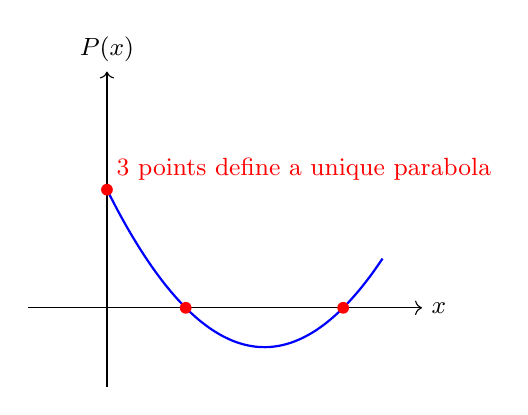
\begin{tikzpicture}[font=\small]
    \draw[->] (-1,0) -- (4,0) node[right] {$x$};
    \draw[->] (0,-1) -- (0,3) node[above] {$P(x)$};
    \draw[smooth, domain=0:3.5, variable=\x, blue, thick] plot ({\x}, {0.5*(\x-1)*(\x-3)});
    \node[red, circle, fill, inner sep=1.5pt] at (1,0) {};
    \node[red, circle, fill, inner sep=1.5pt] at (3,0) {};
    \node[red, circle, fill, inner sep=1.5pt] at (0,1.5) {};
    \node[above right, red] at (0,1.5) {3 points define a unique parabola};
\end{tikzpicture}
\caption{The uniqueness property of polynomials.}
\end{figure}

This property is what allows us to recover lost information. If a message is encoded as points on a polynomial, we only need to recover a sufficient number of those points (any $k$ of them) to reconstruct the entire original message.

\begin{tcolorbox}[title={Example: Reconstructing a Polynomial}]
Suppose we are told that four points, $(-1, 2)$, $(0, 3)$, $(1, -5)$, and $(2, 1)$, lie on a polynomial of degree 3. Our message is encoded in the coefficients $(m_0, m_1, m_2, m_3)$ of this polynomial:
\[ P(x) = m_0 + m_1 x + m_2 x^2 + m_3 x^3 \]
By plugging in each point, we get a system of four linear equations with four unknowns:
\begin{align*}
P(-1) = m_0 - m_1 + m_2 - m_3 &= 2 \\
P(0)  = m_0 &= 3 \\
P(1)  = m_0 + m_1 + m_2 + m_3 &= -5 \\
P(2)  = m_0 + 2m_1 + 4m_2 + 8m_3 &= 1
\end{align*}
Solving this system yields a unique solution for the coefficients: $(m_0, m_1, m_2, m_3) = (3, -4.5, -5.5, 2)$. The fractions highlight a key issue with using real numbers, which we'll address later using finite fields. For now, the crucial insight is that the four points uniquely locked in the polynomial and thus the message.
\end{tcolorbox}


\subsection{The Core Idea: Encoding by Oversampling}
The most intuitive way to understand RS encoding is to view it as "oversampling" a function. We take a message, turn it into a polynomial, and then evaluate that polynomial at more points than are strictly necessary. These extra points are our redundancy.

This leads to a \textbf{systematic} encoding, where the original message is embedded directly within the final codeword. Here's the process:

\begin{enumerate}
    \item \textbf{Interpret the Message as Points:} Take a message block of $k$ symbols, $\mathbf{m} = (m_0, m_1, \dots, m_{k-1})$. Treat these as the $y$-values of a polynomial $P(x)$ at $k$ predefined evaluation points, say $x = 0, 1, \dots, k-1$. This gives us $k$ points: $(0, m_0), (1, m_1), \dots, (k-1, m_{k-1})$.
    \item \textbf{Interpolate to Find the Polynomial:} Find the unique polynomial $P(x)$ of degree at most $k-1$ that passes through these $k$ points.
    \item \textbf{Evaluate to Generate Redundancy:} "Oversample" the function by evaluating $P(x)$ at $n-k$ new points, say $x=k, k+1, \dots, n-1$. These new values are our parity symbols.
    \item \textbf{Form the Codeword:} The final codeword $\mathbf{c}$ is the list of all $n$ evaluations. The first $k$ symbols are the original message, and the next $n-k$ symbols are the redundancy.
\end{enumerate}

\begin{tcolorbox}[title={Example: Systematic RS Encoding}]
Let's encode a message $\mathbf{m}=(3, 1)$ with $k=2$ into a codeword of length $n=4$ over a finite field (we'll use integers for simplicity, but imagine the math is modulo a prime, like 5).
\begin{enumerate}
    \item \textbf{Message as Points:} We treat the message as the values of a polynomial $P(x)$ at $x=0$ and $x=1$. Our points are $(0, 3)$ and $(1, 1)$.
    \item \textbf{Interpolate:} We need to find the unique line (degree $k-1=1$) of the form $P(x) = a_0 + a_1 x$ that passes through these points.
    \begin{itemize}
        \item $P(0) = a_0 = 3$
        \item $P(1) = a_0 + a_1 = 1 \implies 3 + a_1 = 1 \implies a_1 = -2$
    \end{itemize}
    So, our message polynomial is $P(x) = 3 - 2x$.

    \item \textbf{Generate Redundancy:} We oversample by evaluating $P(x)$ at two new points, $x=2$ and $x=3$.
    \begin{itemize}
        \item $P(2) = 3 - 2(2) = -1$
        \item $P(3) = 3 - 2(3) = -3$
    \end{itemize}
    \item \textbf{Form the Codeword:} We concatenate the original message values with the new redundant values.
    \[ \mathbf{c} = (\underbrace{3, 1}_{\text{Message}}, \underbrace{-1, -3}_{\text{Redundancy}}) \]
\end{enumerate}
The final codeword is $(3, 1, -1, -3)$. If this is transmitted and one of the symbols is lost (an erasure), we can still recover the polynomial $P(x)=3-2x$ from any of the remaining three points and regenerate the missing value.
\end{tcolorbox}

\subsection{Why Finite Fields are Essential}
Throughout our examples, we've used integers for simplicity, but you may have noticed a problem: interpolation can produce fractions. Furthermore, the values of the evaluated points can become very large. Digital systems, however, work with fixed-size data types (like bytes) and cannot handle arbitrary fractions or infinite growth. \textbf{Finite fields} (or Galois Fields, GF) solve both problems perfectly.
\begin{enumerate}
    \item \textbf{No Fractions:} In a finite field, division is well-defined and always results in another element of the field. All calculations are exact.
    \item \textbf{Closure:} The result of any addition or multiplication is always another element within the finite set of the field. This prevents numbers from growing too large and ensures that symbols always fit within their designated size (e.g., 8 bits for $\mathbb{F}_{2^8}$).
\end{enumerate}
By constructing polynomials over a finite field like $\mathbb{F}_{256}$, Reed-Solomon codes become perfectly suited for modern digital storage and communication systems.



%%%%%%%%%%%%%%%%%%%%%%%%%%%%%%%%%%%%%%%%%%%%%%%%%%%%%%%
%%%%%%%%%%%%%%%%%%%%%%%%%%%%%%%%%%%%%%%%%%%%%%%%%%%%%%%
%%%%%%%%%%%%%%%%%%%%%%%%%%%%%%%%%%%%%%%%%%%%%%%%%%%%%%%

\section{Proximity Gaps: An All-or-Nothing Property of Codes}

We've explored how codes are built and how they can be used to correct a limited number of errors. But in advanced applications like modern proof systems (e.g., STARKs) and secure multi-party computation, we face a more complex challenge: verifying the integrity of not just one, but a whole \textit{batch} of alleged codewords simultaneously. This leads to a profound structural question about codes, the answer to which has significant real-world consequences.

\subsection{The Motivation: Verifying a Batch of Codewords}
Imagine a scenario where a prover claims that a large set of vectors $\{ \mathbf{u}_0, \mathbf{u}_1, \dots, \mathbf{u}_l \}$ are all valid (or at least very close to valid) Reed-Solomon codewords. Verifying each vector individually would be slow and inefficient. A much faster approach is to ask the prover to combine them into a single vector using random coefficients $r_i$:
\[ \mathbf{u}' = r_0\mathbf{u}_0 + r_1\mathbf{u}_1 + \dots + r_l\mathbf{u}_l \]
The verifier then only needs to check if this single random combination, $\mathbf{u}'$, is close to the code.

This raises a critical security question: \textbf{Is this test sound?} If a malicious prover provides just one vector $\mathbf{u}_i$ that is very far from the code, can they cleverly construct the other vectors such that their random combination $\mathbf{u}'$ almost always looks valid? If so, the test is useless.

For this test to be reliable, we need a guarantee that if even one vector is "far," the random combination will also be "far" with high probability. This is precisely what the theory of \textbf{proximity gaps} provides.

\subsection{The Proximity Gap Phenomenon}
A proximity gap is a powerful "all-or-nothing" principle. It states that for certain codes and structured collections of vectors (like lines or planes, known as affine spaces), there is no middle ground. Every vector in the collection is "close" to being a valid codeword, or almost none are.

\begin{tcolorbox}[breakable, title={Analogy: The Proximity Gap}]
\paragraph{Scenario 1: "All-In" (Correlated Errors)}
Imagine two slightly corrupted vectors, $\mathbf{u}_0$ and $\mathbf{u}_1$, where the errors happen to occur in the \textbf{same position}.
\begin{itemize}
    \item Error in $\mathbf{u}_0$: $(0, 0, 5, 0)$
    \item Error in $\mathbf{u}_1$: $(0, 0, 2, 0)$
\end{itemize}
Any vector on the line between them, $\mathbf{u}_z = \mathbf{u}_0 + z \cdot \mathbf{u}_1$, will have a combined error of $(0, 0, 5+2z, 0)$. Notice that for any value of $z$, the error is still confined to a single position. If one error is correctable, they all are. Thus, \textbf{all} vectors on the line are "close" to the code.

\hrulefill

\paragraph{Scenario 2: "All-Out" (Uncorrelated Errors)}
Now, imagine the errors are in \textbf{different positions}.
\begin{itemize}
    \item Error in $\mathbf{u}_0$: $(5, 0, 0, 0)$
    \item Error in $\mathbf{u}_1$: $(0, 0, 2, 0)$
\end{itemize}
The combined error is $(5, 0, 2z, 0)$. Unless $z=0$, this vector has two errors. If the code can only correct one error, then every vector on the line (except possibly $\mathbf{u}_0$ itself) is now "far" from the code. Thus, \textbf{almost none} of the vectors are "close".

\textbf{The Insight:} The rigid algebraic structure of polynomials prevents widespread, random cancellation of errors. The errors either align perfectly from the start (correlated), or they don't, in which case their combination almost always results in more errors. There is no scenario where roughly half the combinations are close and half are far. This is the essence of the proximity gap.
\end{tcolorbox}

\subsubsection{Formal Definition}
This "all-or-nothing" idea is captured formally in the definition of a proximity gap.

\begin{tcolorbox}[breakable, title={Definition: Proximity Gap}]
A collection of sets $\mathcal{S}$ (e.g., all lines in $\mathbb{F}_q^n$) displays a $(\delta, \varepsilon)$-proximity gap with respect to a code $V$ if for every set $S \in \mathcal{S}$, exactly one of the following is true:
\begin{enumerate}
    \item \textbf{All-In:} Every vector in $S$ is $\delta$-close to the code $V$.
    \[ \Pr_{\mathbf{u} \in S} \left[ d(\mathbf{u}, V) \le \delta n \right] = 1 \]
    \item \textbf{All-Out:} At most a tiny fraction, $\varepsilon$, of vectors in $S$ are $\delta$-close to the code $V$.
    \[ \Pr_{\mathbf{u} \in S} \left[ d(\mathbf{u}, V) \le \delta n \right] \le \varepsilon \]
\end{enumerate}
Here, $\delta$ is the proximity parameter (the fraction of allowed errors), and $\varepsilon$ is the error parameter (a very small number).
\end{tcolorbox}


\subsection{The Main Result: Reed-Solomon Codes Have a Proximity Gap}
The central theorem of the Ben-Sasson et al. paper\cite{ben2023proximity} is that Reed-Solomon codes exhibit exactly this property. This provides the theoretical foundation needed to trust the random linear combination test.

The result is split into two regimes, depending on the fraction of errors $\delta$ we are willing to tolerate, compared to the code's rate $\rho = k/n$.

\begin{tcolorbox}[breakable, title={Theorem (Informal): Proximity Gap for RS Codes}]
The collection of all affine spaces has a strong proximity gap with respect to any Reed-Solomon code $V$. This holds for any fraction of errors $\delta$ up to the Johnson bound.

\paragraph{1. The Unique Decoding Regime ($\delta < \frac{1-\rho}{2}$)}
When the number of errors is small, the gap is extremely sharp. If an affine space is not "All-In", the fraction of close words is at most $\varepsilon = n/q$. For this to be a strong guarantee, we need the field size $q$ to be larger than the block length $n$.

\paragraph{2. The List Decoding (Johnson) Regime ($\frac{1-\rho}{2} \le \delta < 1 - \sqrt{\rho}$)}
Remarkably, the gap still holds for a much larger number of errors. The guarantee is slightly weaker, with the fraction of close words being at most $\varepsilon \approx O(n^2/q)$. To ensure this is a small number, we need a larger field, with $q$ being roughly quadratic in $n$.
\end{tcolorbox}


%%%%%%%%%%%%%%%%%%%%%%%%%%%%%%%%%%%%%%%%%%%%%%%%%%%%%%%
%%%%%%%%%%%%%%%%%%%%%%%%%%%%%%%%%%%%%%%%%%%%%%%%%%%%%%%
%%%%%%%%%%%%%%%%%%%%%%%%%%%%%%%%%%%%%%%%%%%%%%%%%%%%%%%
\subsection{Application: Soundness of the FRI Protocol}

The theory of proximity gaps has a direct and significant application in analyzing the security of modern proof systems. Specifically, it provides the mathematical foundation for the soundness of the FRI protocol\cite{ben2018fast} (Fast Reed-Solomon Interactive Oracle Proof of Proximity), which is a core component of transparent and quantum-resistant proof systems like STARKs.

\subsubsection{The FRI Protocol: A Recursive Low-Degree Test}
The primary function of the FRI protocol is to perform a \textbf{low-degree test}. In this context, a prover possesses a large dataset, represented as a function $f^{(0)}$ over a domain $D_0$, and asserts that this function is the evaluation of a low-degree polynomial $P_0(x)$ (i.e., that $f^{(0)}$ is a Reed-Solomon codeword). A verifier must be able to check this claim with high confidence by querying only a small number of points from the dataset.

FRI accomplishes this through a recursive process known as "folding." In each round, the prover reduces a given function to a new, smaller function, effectively halving its associated degree and domain size.

\begin{tcolorbox}[breakable, title={The FRI Folding Step}]
In each round $i$, the protocol begins with a function $f^{(i)}$ that is asserted to be of a certain low degree.
\begin{enumerate}
    \item The prover splits $f^{(i)}$ into two components, often based on the even and odd coefficients of its polynomial representation:
    \[ f^{(i)}(x) = f^{(i)}_{\text{even}}(x^2) + x \cdot f^{(i)}_{\text{odd}}(x^2) \]
    \item The verifier provides a random challenge scalar, $z_i \in \mathbb{F}_q$.
    \item The prover uses this challenge to form a random linear combination of the two components. This defines the function for the next round:
    \[ f^{(i+1)}(y) = f^{(i)}_{\text{even}}(y) + z_i \cdot f^{(i)}_{\text{odd}}(y) \]
    The domain of $f^{(i+1)}$ is the set of squared elements from the previous domain, thus its size is halved.
\end{enumerate}
This recursive process continues until the function is small enough for the verifier to check completely by reading all of its values.
\end{tcolorbox}

\subsubsection{The Soundness Argument}
The security analysis of the FRI protocol involves two properties:
\begin{itemize}
    \item \textbf{Completeness:} An honest prover, starting with a true low-degree polynomial $f^{(0)}$, will always pass the verification. This property is straightforward to show, as the folding process preserves the low-degree nature of the function at each step. This is often referred to as the "top-down" direction of the argument.
    \item \textbf{Soundness:} A dishonest prover, starting with a function $f^{(0)}$ that is far from any low-degree polynomial, will be caught with high probability. Proving this is more complex. It requires a "bottom-up" argument.
\end{itemize}
The core of the soundness proof is to show that the low-degree property propagates backwards up the recursive ladder. If the verifier is convinced that the final function $f^{(r)}$ is low-degree, it must follow that the initial function $f^{(0)}$ was also close to being low-degree.

\subsubsection{The Role of the Proximity Gap in the Soundness Proof}
The potential vulnerability in the soundness argument lies in the folding step. A malicious prover could attempt to construct functions $f^{(i)}_{\text{even}}$ and $f^{(i)}_{\text{odd}}$ that are both far from being low-degree, but whose random combination,
\[ f^{(i+1)} = f^{(i)}_{\text{even}} + z_i \cdot f^{(i)}_{\text{odd}} \]
is close to a low-degree polynomial for a non-negligible fraction of the verifier's random challenges $z_i$.

This is precisely the scenario that the proximity gap theorem for Reed-Solomon codes demonstrates is not possible. The set of functions $\{ f^{(i)}_{\text{even}} + z \cdot f^{(i)}_{\text{odd}} \mid z \in \mathbb{F}_q \}$ forms an affine line. The proximity gap theorem dictates that such a line must be either "All-In" (all functions are close to the code) or "All-Out" (almost no functions are close). A middle ground, where a significant fraction but not all functions are close, does not exist.

\begin{tcolorbox}[breakable, title={How the Proximity Gap Secures FRI}]
The proximity gap provides the critical logical step in the bottom-up soundness argument.
\begin{enumerate}
    \item The verifier confirms that the final function, $f^{(r)}$, is a low-degree polynomial.
    \item The verifier then proceeds backwards to round $i$. He is convinced that $f^{(i+1)}$ has high agreement with a low-degree polynomial (a codeword).
    \item This means that for the prover's chosen $f^{(i)}_{\text{even}}$ and $f^{(i)}_{\text{odd}}$, their combination using the random challenge $z_i$ was close to a codeword.
    \item For the prover's attack to be successful, this would need to hold true for a significant fraction of possible challenges $z_i$.
    \item The Proximity Gap Theorem states that if the line of functions $\{ f^{(i)}_{\text{even}} + z \cdot f^{(i)}_{\text{odd}} \}$ is close to the code for more than a tiny fraction $\varepsilon$ of challenges, it must be the "All-In" case.
    \item The "All-In" case implies a strong structural property known as \textbf{correlated agreement}: the functions $f^{(i)}_{\text{even}}$ and $f^{(i)}_{\text{odd}}$ must themselves be close to low-degree polynomials, with their errors located in the same positions.
    \item This correlated agreement is the necessary condition to prove that the parent function, $f^{(i)}$, was also close to being a low-degree polynomial.
\end{enumerate}
By providing this inferential link at each recursive step, the proximity gap guarantees that the low-degree property propagates from the final function all the way back to the initial one. This ensures the soundness of the random linear combination check at the heart of FRI, which in turn allows the protocol to achieve high security with few queries, leading to smaller proof sizes and faster verification times.
\end{tcolorbox}


\subsubsection{From Tighter Soundness to Smaller Proofs}
The primary goal of cryptographic proof systems like STARKs is to achieve a high level of security (e.g., 128 bits) as efficiently as possible. Efficiency is measured by the proof size and verifier computation time. The soundness analysis of FRI, backed by the proximity gap theorem, directly impacts this efficiency.

The connection is based on the relationship between security, queries, and proof size:
\begin{itemize}
    \item \textbf{Proof Size depends on Queries:} A significant portion of a STARK proof consists of Merkle authentication paths that substantiate the prover's answers to the verifier's random queries. Therefore, the total proof size is directly proportional to the number of queries performed.
    \item \textbf{Queries depend on Soundness:} To reach a target security level, the verifier must perform enough queries to reduce the probability of accepting a false proof to a negligible amount (e.g., $2^{-128}$). The number of queries needed depends on the \textit{soundness error} of the protocol — that is, how effective each individual query is at catching a malicious prover.
\end{itemize}

This is where the proximity gap theorem provides a crucial improvement. Older analyses of the FRI protocol had looser bounds on the soundness error, suggesting that each query was only moderately effective at detecting fraud. To compensate, a large number of queries were required to achieve the desired security level, leading to larger proofs.

The proximity gap theorem provides a \textbf{tighter soundness analysis}. It proves that the random linear combination check at the heart of FRI is exceptionally reliable. This means each query is far more powerful at detecting inconsistencies than previously understood.

In summary, because the proximity gap provides a stronger guarantee on the soundness of FRI, fewer queries are needed to achieve the same level of cryptographic security. This directly translates to fewer Merkle paths in the final STARK proof, resulting in a smaller proof size and faster verification time.



%%%%%%%%%%%%%%%%%%%%%%%%%%%%%%%%%%%%%%%%%%%%%%%%%%%%%%%
%%%%%%%%%%%%%%%%%%%%%%%%%%%%%%%%%%%%%%%%%%%%%%%%%%%%%%%
%%%%%%%%%%%%%%%%%%%%%%%%%%%%%%%%%%%%%%%%%%%%%%%%%%%%%%%

\section{Proof of the Proximity Gap (Unique Decoding Regime)}

This section details the proof for the proximity gap of Reed-Solomon codes in the unique decoding regime. The proof demonstrates that if a significant fraction of vectors on an affine line are close to a Reed-Solomon code, then the vectors defining the line must share a strong algebraic structure. This structure, in turn, forces the entire line to be close to the code.

\subsection{The Goal and the Strategy}
The formal statement we aim to prove, based on Theorem 4.1 in Ben-Sasson et al.\cite{ben2023proximity}, is as follows:

\begin{tcolorbox}[breakable, title={Theorem to Prove (Correlated Agreement)}]
Let $V$ be a Reed-Solomon code of degree $k$ over a domain $D \subset \mathbb{F}_q$. Let $\{\mathbf{u}_0 + z \cdot \mathbf{u}_1 \mid z \in \mathbb{F}_q\}$ be an affine line of vectors.

If the set $S = \{z \in \mathbb{F}_q \mid d(\mathbf{u}_0 + z \cdot \mathbf{u}_1, V) \le \delta n\}$ is sufficiently large (specifically, $|S| > k+1$), then there must exist two codewords, $\mathbf{v}_0, \mathbf{v}_1 \in V$, such that $\mathbf{u}_0$ and $\mathbf{v}_0$ agree on a large fraction of coordinates, and $\mathbf{u}_1$ and $\mathbf{v}_1$ agree on that \textit{same} large fraction of coordinates. This property is known as \textbf{correlated agreement}.
\end{tcolorbox}

\paragraph{The Proof Strategy}
The core of the proof is a shift in perspective. Instead of analyzing each of the $|S|$ "close" vectors individually, we analyze the entire line simultaneously using a higher level of algebraic abstraction.
\begin{enumerate}
    \item \textbf{Create a Formal Object:} We represent the entire affine line as a single \textit{formal vector} $\mathbf{w}(x)$ whose entries are linear polynomials in a formal variable $Z$. This vector is defined over a \textbf{function field} $\mathbb{F}_q(Z)$.
    \[ \mathbf{w}(x) = \mathbf{u}_0(x) + Z \cdot \mathbf{u}_1(x) \]
    \item \textbf{Decode the Formal Object:} We run a classic Reed-Solomon decoding algorithm, the Berlekamp-Welch algorithm, on this single formal vector $\mathbf{w}$.
    \item \textbf{Deduce Structure:} We show that the success of the decoder on many concrete instances (for $Z=z$ where $z \in S$) implies that the decoder must also succeed on the formal object. The output of this formal decoding reveals the correlated agreement between the original vectors $\mathbf{u}_0$ and $\mathbf{u}_1$.
\end{enumerate}

\subsection{The Toolkit: Algebraic Decoders and Lemmas}
The proof relies on two key algebraic tools.


%%%%%%%%%%%%%%%%%%%%%%%%%%%%%%%%%%%%%%%%%%%%%%%%%%%%%%%
%%%%%%%%%%%%%%%%%%%%%%%%%%%%%%%%%%%%%%%%%%%%%%%%%%%%%%%
%%%%%%%%%%%%%%%%%%%%%%%%%%%%%%%%%%%%%%%%%%%%%%%%%%%%%%%

\subsubsection{Tool 1: The Berlekamp-Welch Algorithm}
The Berlekamp-Welch (BW) algorithm is a method for the unique decoding of Reed-Solomon codes. Its objective is to recover the original low-degree polynomial $P(X)$ from a received word $\mathbf{w}$ that may contain a limited number of errors at unknown locations.

The main challenge in error correction is that the locations of the errors are unknown. The BW algorithm's sidesteps this problem by creating a new equation that holds true for \textit{all} positions, whether they are corrupted or not. It achieves this by turning the non-linear problem of finding error locations into a system of linear equations.

\paragraph{The Auxiliary Polynomials}
The algorithm introduces two auxiliary polynomials whose coefficients are the unknowns we need to solve for:
\begin{itemize}
    \item An \textbf{Error-Locator Polynomial}, $A(X)$. This is a polynomial of degree $t$ (the number of errors the code can correct) whose roots are the locations of the corrupted symbols. It is defined as:
    \[ A(X) = (X - e_1)(X - e_2)\dots(X - e_t) \]
    where $e_1, \dots, e_t$ are the positions of the errors. Crucially, we do not know these positions in advance; the algorithm will find the coefficients of $A(X)$ for us, which implicitly reveals the error locations. The defining property of this polynomial is that $A(x) = 0$ if and only if position $x$ contains an error.

    \item A \textbf{Codeword-Evaluator Polynomial}, $B(X)$. This polynomial is defined as the product of the original (and unknown) message polynomial $P(X)$ and the error-locator polynomial $A(X)$:
    \[ B(X) = P(X) \cdot A(X) \]
\end{itemize}

\paragraph{The Key Equation}
Using these definitions, the BW algorithm establishes an equation that is valid for every point $x$ in the evaluation domain $D$, where $\mathbf{w}(x)$ is the received symbol at that position:
\[ A(x) \cdot \mathbf{w}(x) = B(x) \]
This identity holds universally due to the following case analysis:
\begin{enumerate}
    \item \textbf{Case 1: Position $x$ is correct.} By definition, the received symbol is the same as the original, so $\mathbf{w}(x) = P(x)$. The equation becomes $A(x) \cdot P(x) = B(x)$, which is true by the definition of $B(X)$.
    \item \textbf{Case 2: Position $x$ is corrupted.} In this case, $\mathbf{w}(x) \neq P(x)$. However, because $x$ is an error location, it must be a root of the error-locator polynomial, meaning $A(x) = 0$. The equation becomes $0 \cdot \mathbf{w}(x) = 0$, which is always true.
\end{enumerate}
Then, the master equation, $A(x)\mathbf{w}(x) = B(x)$, holds for every position, effectively masking the errors.

\paragraph{Solving the System}
The equation $A(x)\mathbf{w}(x) = B(x)$ is a \textit{linear} equation in the unknown coefficients of $A(X)$ and $B(X)$. By evaluating this equation at every point $x \in D$ (of which there are $n$), we generate a system of $n$ linear equations. The number of unknowns is the sum of the unknown coefficients in $A(X)$ and $B(X)$. For a code that corrects $t$ errors, this gives us just enough equations to solve for the unknowns uniquely.


\begin{tcolorbox}[breakable, title={The Berlekamp-Welch Algorithm: A Summary}]
The goal is to recover the original polynomial $P(X)$ from a received word $\mathbf{w}$.
\begin{enumerate}
    \item \textbf{Set up the System:} Construct a system of $n$ linear equations by asserting that $A(x) \cdot \mathbf{w}(x) = B(x)$ for every position $x$ in the domain. The variables are the unknown coefficients of the polynomials $A(X)$ and $B(X)$.
    \item \textbf{Solve for the Polynomials:} Solve the linear system to find the unique coefficients of the error-locator $A(X)$ and the evaluator $B(X)$.
    \item \textbf{Recover the Message:} The original message polynomial is recovered by performing polynomial division:
    \[ P(X) = \frac{B(X)}{A(X)} \]
\end{enumerate}
If $\mathbf{w}$ is indeed close to a low-degree polynomial, a non-zero solution for $A(X)$ and $B(X)$ is guaranteed to exist, and $A(X)$ is guaranteed to divide $B(X)$ without a remainder.
\end{tcolorbox}

\paragraph{A Closer Look: The System of Equations}
The equation $A(x) \cdot \mathbf{w}(x) = B(x)$ is linear in the unknown coefficients of $A(X)$ and $B(X)$. To understand the setup, let's count these unknown coefficients.

\paragraph{Counting the Unknowns}
Assume the code can correct up to $t$ errors and the message polynomial $P(X)$ has degree less than $k$.
\begin{itemize}
    \item For $A(X)$: This polynomial must have a root at each of the $t$ error locations. Its degree is therefore exactly $t$. A polynomial of degree $t$ has $t+1$ coefficients. By convention, we set the leading coefficient to 1 (making it \textit{monic}), which leaves exactly $t$ unknown coefficients.
    \[ A(X) = \underbrace{1 \cdot X^t}_{\text{Known}} + \underbrace{a_{t-1}X^{t-1} + \dots + a_0}_{\text{t unknown coefficients}}\]
    \item For $B(X)$: This polynomial is the product $B(X) = P(X) \cdot A(X)$. The degree of a product is the sum of the degrees:
    \[ \deg(B) = \deg(P) + \deg(A) \le (k-1) + t = k+t-1 \]
    A polynomial of degree $k+t-1$ has $k+t$ coefficients in total:
    \[ B(X) = \underbrace{b_{k+t-1}X^{k+t-1} + \dots + b_0}_{\text{k+t unknown coefficients}} \]
\end{itemize}
In total, we have $t + (k+t) = k+2t$ unknown coefficients to solve for.

\paragraph{Constructing the Equations}
For each of the $n$ received points $(x_i, \mathbf{w}_i)$, we write down our key equation. This gives us $n$ linear equations, one of which is shown below:
\[ \underbrace{(b_{k+t-1}x_i^{k+t-1} + \dots + b_0)}_{\text{Linear expression in unknown } b_j\text{'s}} = \mathbf{w}_i \cdot \underbrace{(x_i^t + a_{t-1}x_i^{t-1} + \dots + a_0)}_{\text{Linear expression in unknown } a_j\text{'s}} \]
Since the code is designed such that $n \ge k+2t$, we have at least as many equations as unknowns, which allows us to find a unique solution for the coefficients.

%%%%%%%%%%%%%%%%%%%%%%%%%%%%%%%%%%%%%%%%%%%%%%%%%%%%%%%
%%%%%%%%%%%%%%%%%%%%%%%%%%%%%%%%%%%%%%%%%%%%%%%%%%%%%%%
%%%%%%%%%%%%%%%%%%%%%%%%%%%%%%%%%%%%%%%%%%%%%%%%%%%%%%%

\subsubsection{Tool 2: The Polishchuk-Spielman Lemma}
This lemma provides the logical bridge from a property observed in many specific instances to a property that must hold formally and universally. It allows us to "lift" a conclusion from a collection of concrete observations to a single, abstract algebraic truth.

\paragraph{Intuition: From Slices to the Whole}
Imagine a two-variable polynomial, $B(X,Z)$, as a surface. When we fix the value of $Z$ to a specific constant, $z$, we are taking a vertical "slice" of that surface, which results in a simple one-variable curve, $B(X,z)$.

The situation in our proof is that we have two such surfaces, $A(X,Z)$ and $B(X,Z)$. We don't know their formal relationship, but we do observe that for many different slices (i.e., for many values of $z$), the curve $A(X,z)$ divides the curve $B(X,z)$. It is highly unlikely for this divisibility to occur repeatedly by coincidence. The Polishchuk-Spielman lemma formalizes this intuition, stating that if this pattern holds for a sufficient number of slices, it cannot be an accident.

\begin{tcolorbox}[breakable, title={The Polishchuk-Spielman Lemma (Principle)}]
If the univariate polynomial $A(X,z)$ divides $B(X,z)$ for a sufficiently large number of distinct values of $z$, then the bivariate polynomial $A(X,Z)$ must formally divide $B(X,Z)$. This means there exists a third polynomial, $P(X,Z)$, such that:
\[ B(X,Z) = A(X,Z) \cdot P(X,Z) \]

\begin{center}
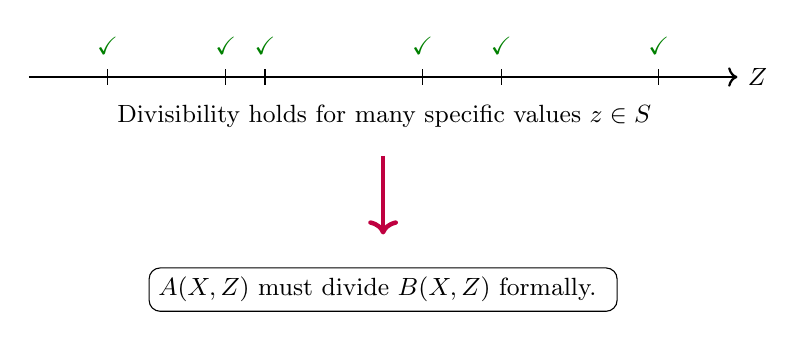
\begin{tikzpicture}[font=\small]
    % Draw the Z-axis
    \draw[->, thick] (0,0) -- (9,0) node[right] {$Z$};
    
    % Mark points on the axis where divisibility holds
    \foreach \x in {1, 2.5, 3, 5, 6, 8} {
        \draw (\x, 0.1) -- (\x, -0.1);
        \node[green!50!black] at (\x, 0.4) {$\checkmark$};
    }
    \node[anchor=west] at (1, -0.5) {Divisibility holds for many specific values $z \in S$};
    
    % Implication arrow
    \draw[->, ultra thick, purple] (4.5, -1) -- (4.5, -2);
    
    % Formal conclusion
    \node[draw, rounded corners, align=center] at (4.5, -2.7) {
        $A(X,Z)$ must divide $B(X,Z)$ formally.
    };
\end{tikzpicture}
\end{center}
This principle allows us to deduce a strong, formal algebraic property from a collection of individual observations.
\end{tcolorbox}


%%%%%%%%%%%%%%%%%%%%%%%%%%%%%%%%%%%%%%%%%%%%%%%%%%%%%%%
%%%%%%%%%%%%%%%%%%%%%%%%%%%%%%%%%%%%%%%%%%%%%%%%%%%%%%%
%%%%%%%%%%%%%%%%%%%%%%%%%%%%%%%%%%%%%%%%%%%%%%%%%%%%%%%



\subsection{The Proof}
With these tools, the proof proceeds as follows.


%%%%%%%%%%%%%%%%%%%%%%%%%%%%%%%%%%%%%%%%%%%%%%%%%%%%%%%
%%%%%%%%%%%%%%%%%%%%%%%%%%%%%%%%%%%%%%%%%%%%%%%%%%%%%%%
%%%%%%%%%%%%%%%%%%%%%%%%%%%%%%%%%%%%%%%%%%%%%%%%%%%%%%%


\subsubsection{Step 1: Constructing a Formal Solution with Berlekamp-Welch}
Our first step is to apply the Berlekamp-Welch algorithm to our formal word $\mathbf{w}(x) = \mathbf{u}_0(x) + Z \cdot \mathbf{u}_1(x)$. This requires us to find two formal polynomials, $A(X,Z)$ and $B(X,Z)$, that satisfy the key equation for all $x \in D$:
\[ A(x, Z) \cdot \big(\mathbf{u}_0(x) + Z \cdot \mathbf{u}_1(x)\big) = B(x, Z) \]
The challenge is to prove that a non-trivial solution (where $A$ and $B$ are not both the zero polynomial) is guaranteed to exist.

\paragraph{From Polynomial Equation to Linear System}
The equation above might seem complex, but it's actually a system of linear equations in disguise. The true \textit{unknowns} are the coefficients of the polynomials $A(X,Z)$ and $B(X,Z)$. These coefficients are not simple numbers; they are polynomials in the formal variable $Z$. Let's denote them $A_j(Z)$ and $B_j(Z)$.

For each evaluation point $x_i \in D$, we get one linear equation. If we have $n$ points in our domain, we have a system of $n$ linear equations. This can be written in matrix form:
\[ \mathbf{M}(Z) \cdot \mathbf{c}(Z) = \mathbf{0} \]
Here, $\mathbf{c}(Z)$ is a vector containing all the unknown coefficient polynomials, and $\mathbf{M}(Z)$ is a large matrix whose entries are themselves polynomials in $Z$.

\begin{tcolorbox}[breakable, title={Illustration: A Small Example of the Matrix $\mathbf{M}(Z)$}]
Let's consider a small code with the following parameters:
\begin{itemize}
    \item A message polynomial of degree at most $k-1=1$ (so dimension $k=2$).
    \item The ability to correct $t=1$ error.
    \item An evaluation domain of $n=4$ points, $\{x_1, x_2, x_3, x_4\}$.
\end{itemize}
The Berlekamp-Welch algorithm needs to find the unknown polynomials $A(X,Z)$ and $B(X,Z)$. Let's determine their form:
\begin{itemize}
    \item $A(X,Z)$ is the error-locator of degree $t=1$. It has the form $A(X,Z) = A_1(Z)X + A_0(Z)$.
    \item $B(X,Z)$ is the product $P(X)A(X,Z)$. Its degree is at most $(k-1)+t = 1+1=2$. It has the form $B(X,Z) = B_2(Z)X^2 + B_1(Z)X + B_0(Z)$.
\end{itemize}
The unknowns are the five coefficient functions: $\{A_1(Z), A_0(Z), B_2(Z), B_1(Z), B_0(Z)\}$.

The key equation is $A(x,Z) \cdot \mathbf{w}(x,Z) - B(x,Z) = 0$. For a single point $x_i$, this expands to:
\[ \underbrace{\left( A_1(Z)x_i + A_0(Z) \right)}_{\text{Evaluated } A} \cdot \underbrace{\left( \mathbf{u}_0(x_i) + Z\mathbf{u}_1(x_i) \right)}_{\text{Formal word } \mathbf{w}_i(Z)} - \underbrace{\left( B_2(Z)x_i^2 + B_1(Z)x_i + B_0(Z) \right)}_{\text{Evaluated } B} = 0 \]
By rearranging and grouping the five unknown coefficient functions, we get a linear equation. We generate one such equation for each of the $n=4$ points. This gives us a system of 4 linear equations for 5 unknowns, which can be written in matrix form $\mathbf{M}(Z) \cdot \mathbf{c}(Z) = \mathbf{0}$:
\[
\underbrace{
\begin{pmatrix}
x_1 \mathbf{w}_1(Z) & \mathbf{w}_1(Z) & -x_1^2 & -x_1 & -1 \\
x_2 \mathbf{w}_2(Z) & \mathbf{w}_2(Z) & -x_2^2 & -x_2 & -1 \\
x_3 \mathbf{w}_3(Z) & \mathbf{w}_3(Z) & -x_3^2 & -x_3 & -1 \\
x_4 \mathbf{w}_4(Z) & \mathbf{w}_4(Z) & -x_4^2 & -x_4 & -1
\end{pmatrix}
}_{\text{The } 4 \times 5 \text{ matrix } \mathbf{M}(Z)}
\cdot
\begin{pmatrix}
A_1(Z) \\ A_0(Z) \\ B_2(Z) \\ B_1(Z) \\ B_0(Z)
\end{pmatrix}
=
\begin{pmatrix}
0 \\ 0 \\ 0 \\ 0
\end{pmatrix}
\]
In this specific example, since the matrix has more columns (5 unknowns) than rows (4 equations), linear algebra guarantees that a non-trivial (non-zero) solution must exist.

In the general proof, the matrix is not always "wide". For cases where the number of equations is greater than or equal to the number of unknowns, the more powerful determinant argument (using the "Too Many Roots" principle) is required to prove that the matrix is rank-deficient and that a non-trivial formal solution still exists.
\end{tcolorbox}



\begin{tcolorbox}[breakable, title={Example: The General Case (A "Tall" or Square Matrix)}]
Let's now consider a more general case where the simple "more columns than rows" argument does not apply. Imagine a code with these parameters:
\begin{itemize}
    \item Message polynomial of degree at most $k-1=1$ (dimension $k=2$).
    \item Ability to correct $t=1$ error.
    \item An evaluation domain of $n=5$ points, $\{x_1, \dots, x_5\}$.
\end{itemize}

\paragraph{Counting Unknowns and Equations}
The unknown polynomials are:
\begin{itemize}
    \item $A(X,Z) = A_1(Z)X + A_0(Z)$, with 2 unknown coefficient functions.
    \item $B(X,Z)$, with $\deg(B) \le (k-1)+t = 1+1=2$. So, $B(X,Z) = B_2(Z)X^2 + B_1(Z)X + B_0(Z)$, with 3 unknown coefficient functions.
\end{itemize}
The total number of unknown functions is $2+3=5$. The number of equations is the number of evaluation points, $n=5$.

\paragraph{The Matrix System}
The key equation is $A(x,Z) \cdot \mathbf{w}(x,Z) - B(x,Z) = 0$. For a single point $x_i$, this expands to:
\[ \underbrace{\left( A_1(Z)x_i + A_0(Z) \right)}_{\text{Evaluated } A} \cdot \underbrace{\left( \mathbf{u}_0(x_i) + Z\mathbf{u}_1(x_i) \right)}_{\text{Formal word } \mathbf{w}_i(Z)} - \underbrace{\left( B_2(Z)x_i^2 + B_1(Z)x_i + B_0(Z) \right)}_{\text{Evaluated } B} = 0 \]
Writing one such equation for each of the 5 points gives us a \textbf{square} $5 \times 5$ system of linear equations, $\mathbf{M}(Z) \cdot \mathbf{c}(Z) = \mathbf{0}$:
\[
\underbrace{
\begin{pmatrix}
x_1 \mathbf{w}_1(Z) & \mathbf{w}_1(Z) & -x_1^2 & -x_1 & -1 \\
x_2 \mathbf{w}_2(Z) & \mathbf{w}_2(Z) & -x_2^2 & -x_2 & -1 \\
x_3 \mathbf{w}_3(Z) & \mathbf{w}_3(Z) & -x_3^2 & -x_3 & -1 \\
x_4 \mathbf{w}_4(Z) & \mathbf{w}_4(Z) & -x_4^2 & -x_4 & -1 \\
x_5 \mathbf{w}_5(Z) & \mathbf{w}_5(Z) & -x_5^2 & -x_5 & -1
\end{pmatrix}
}_{\text{The } 5 \times 5 \text{ matrix } \mathbf{M}(Z)}
\cdot
\begin{pmatrix}
A_1(Z) \\ A_0(Z) \\ B_2(Z) \\ B_1(Z) \\ B_0(Z)
\end{pmatrix}
=
\begin{pmatrix}
0 \\ 0 \\ 0 \\ 0 \\ 0
\end{pmatrix}
\]

\paragraph{The Need for the Determinant Argument}
In this case, because the matrix is square, a non-trivial solution is \textbf{not} automatically guaranteed. From linear algebra, a non-trivial solution exists if and only if the determinant of the matrix is zero:
\[ \det(\mathbf{M}(Z)) = 0 \]
This is precisely why the proof must show that this determinant polynomial, $R(Z) = \det(\mathbf{M}(Z))$, is identically zero. This is accomplished using the "Too Many Roots" principle, which handles all cases, whether the matrix is wide, square, or tall.
\end{tcolorbox}






\paragraph{Proving a Solution Exists: The Determinant Argument}
From linear algebra, a homogeneous system of equations like $\mathbf{M}(Z) \cdot \mathbf{c}(Z) = \mathbf{0}$ has a non-trivial solution if and only if its matrix $\mathbf{M}(Z)$ is \textbf{rank-deficient}. This means the rows (or columns) are not all linearly independent; there is some redundancy in the equations. The standard way to check for rank deficiency is to compute the determinants of all the largest possible square submatrices (known as maximal minors). If all of these determinants are zero, the matrix is rank-deficient and a solution is guaranteed.

Our goal is therefore to prove that for our formal matrix $\mathbf{M}(Z)$, the determinant of every maximal square submatrix is identically the zero polynomial. We can prove this for any such determinant, which we'll call $R(Z)$, by using what I will call the "Too Many Roots" principle (for ease of understanding and identification).

\begin{tcolorbox}[breakable, title={The "Too Many Roots" Principle}]
A non-zero, one-variable polynomial of degree $d$ can have at most $d$ distinct roots.
\begin{center}
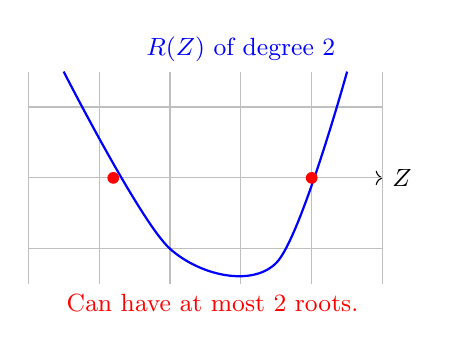
\begin{tikzpicture}[font=\small, scale=0.9]
    \draw[->] (-1,0) -- (4,0) node[right] {$Z$};
    \draw[gray!50] (-1,-1.5) grid (4,1.5);
    \draw[blue, thick, smooth] plot coordinates {(-0.5, 1.5) (1, -1) (2.5, -1.2) (3.5, 1.5)};
    \node[blue, above] at (2,1.5) {$R(Z)$ of degree 2};
    \node[red, circle, fill, inner sep=1.5pt] at (0.2, 0) {};
    \node[red, circle, fill, inner sep=1.5pt] at (3, 0) {};
    \node[red, below] at (1.6, -1.5) {Can have at most 2 roots.};
\end{tikzpicture}
\end{center}
\textbf{The Implication:} If we find that a polynomial of degree at most $d$ actually has $d+1$ or more roots, it must be the \textbf{zero polynomial}, $R(Z) \equiv 0$.
\end{tcolorbox}

The proof follows a clear, three-step logical chain:
\begin{enumerate}
    \item \textbf{The Determinant is a Low-Degree Polynomial:}
    Since the entries of the formal matrix $\mathbf{M}(Z)$ are polynomials in $Z$, the determinant of any of its square submatrices, $R(Z)$, is also a polynomial in $Z$. A careful analysis of the matrix structure, as shown in the paper, reveals that the degree of this polynomial is low. Specifically, it is at most $t+1$, where $t$ is the number of errors the code can correct.
    \[ \deg(R(Z)) \le t+1 \]

    \item \textbf{The "Good" Set Provides Many Roots:}
    This is the important step that connects our initial assumption to the formal system. We assumed that for every $z$ in our "good" set $S$, the concrete word $\mathbf{u}_0 + z \cdot \mathbf{u}_1$ is close to a codeword. The Berlekamp-Welch algorithm guarantees that the corresponding concrete system, $\mathbf{M}(z) \cdot \mathbf{c} = \mathbf{0}$, has a non-trivial solution for each of these $z$'s.

    This can only be true if each concrete matrix $\mathbf{M}(z)$ is rank-deficient, which means the determinant of our chosen square submatrix, when evaluated at $z$, must be zero.
    \[ \underbrace{R(z) = 0}_{\text{The determinant is zero...}} \quad \underbrace{\text{for all } z \in S}_{\text{...at every "good" point.}} \]
    This gives us a powerful piece of information: every single element in the set $S$ must be a root of the polynomial $R(Z)$.

    \item \textbf{Applying the Principle to Prove $R(Z) \equiv 0$:}
    The final step brings the previous two points together. The setup of the theorem requires that the size of our "good" set is greater than the maximum possible degree of the determinant polynomial, i.e., $|S| > t+1$. We are therefore faced with the following situation:
    \[ \text{A polynomial } R(Z) \text{ with } \underbrace{\deg(R(Z)) \le t+1}_{\text{Low Degree}} \text{ that has } \underbrace{|S| > t+1}_{\text{Many Roots}} \]
    According to the "Too Many Roots" principle, this is impossible unless $R(Z)$ is the zero polynomial.
\end{enumerate}
Since this argument holds for any maximal square submatrix of $\mathbf{M}(Z)$, we conclude that the formal matrix is rank-deficient. Therefore, a formal, non-trivial solution for $A(X,Z)$ and $B(X,Z)$ is guaranteed to exist.


\begin{tcolorbox}[breakable, title={Full Example: Proving a Formal Solution Exists}]
Let's walk through the entire process with a numerical example.

\paragraph{1. The Setup}
Suppose we are working over the finite field $\mathbb{F}_5 = \{0,1,2,3,4\}$. We have an affine line of words defined by $\mathbf{u}_0$ and $\mathbf{u}_1$ over the domain $D=\{0,1,2,3\}$ ($n=4$).
\begin{itemize}
    \item $\mathbf{u}_0 = (1, 0, 3, 0)$
    \item $\mathbf{u}_1 = (3, 2, 2, 1)$
\end{itemize}
Our assumption is that for a "good" set of values $S$, the word $\mathbf{w}_z = \mathbf{u}_0 + z \cdot \mathbf{u}_1$ is close to the Reed-Solomon code of degree $k-1=1$. Let's say we have found three such values, $S=\{1,2,3\}$. (This corresponds to $t=1$ error correction, where we need $|S| > t+1$, so $3 > 2$).

\paragraph{2. The Formal Matrix $\mathbf{M}(Z)$}
We set up the Berlekamp-Welch system for our formal word $\mathbf{w}(x,Z) = \mathbf{u}_0(x) + Z\mathbf{u}_1(x)$. With $n=4, k=2, t=1$, we get a $4 \times 4$ square system $\mathbf{M}(Z)\cdot\mathbf{c}(Z) = \mathbf{0}$. The entries of $\mathbf{M}(Z)$ are polynomials in $Z$:
\[
\mathbf{M}(Z) = 
\begin{pmatrix}
x_1 \mathbf{w}_1(Z) & \mathbf{w}_1(Z) & -x_1 & -1 \\
x_2 \mathbf{w}_2(Z) & \mathbf{w}_2(Z) & -x_2 & -1 \\
x_3 \mathbf{w}_3(Z) & \mathbf{w}_3(Z) & -x_3 & -1 \\
x_4 \mathbf{w}_4(Z) & \mathbf{w}_4(Z) & -x_4 & -1
\end{pmatrix}
=
\begin{pmatrix}
0 & 1+3Z & 0 & -1 \\
1(0+2Z) & 0+2Z & -1 & -1 \\
2(3+2Z) & 3+2Z & -2 & -1 \\
3(0+1Z) & 0+1Z & -3 & -1
\end{pmatrix}
\]

\paragraph{3. The Determinant as a Polynomial $R(Z)$}
To prove a formal solution exists, we must show that $\det(\mathbf{M}(Z)) = 0$. This determinant, $R(Z)$, is a polynomial in $Z$. By inspecting the matrix, we can see the highest power of $Z$ in any entry is 1. The determinant calculation involves products of entries, and in a $4 \times 4$ matrix, the highest possible degree is bounded. In this case, it can be shown that $\deg(R(Z)) \le t+1 = 2$.

\paragraph{4. Finding Roots of $R(Z)$ using the set $S$}
This is the key step. We know that for every $z \in S=\{1,2,3\}$, the concrete system has a solution, which means the determinant of the concrete matrix $\mathbf{M}(z)$ must be zero. Let's check for $z=1$:
\[ \mathbf{M}(1) = \begin{pmatrix} 0 & 4 & 0 & -1 \\ 2 & 2 & -1 & -1 \\ 0 & 0 & -2 & -1 \\ 3 & 1 & -3 & -1 \end{pmatrix} \pmod 5 \]
The determinant of this matrix is indeed 0. Therefore, $R(1)=0$, and $Z=1$ is a root of $R(Z)$.

If we do the same for $z=2$ and $z=3$, we would find that $\det(\mathbf{M}(2))=0$ and $\det(\mathbf{M}(3))=0$. So, $Z=2$ and $Z=3$ are also roots.

\paragraph{5. Applying the "Too Many Roots" Principle}
We have now established the following facts:
\begin{itemize}
    \item $R(Z)$ is a polynomial with $\deg(R(Z)) \le 2$.
    \item $R(Z)$ has at least 3 roots (at $Z=1, 2, 3$).
\end{itemize}
Since the number of roots (3) is greater than the maximum possible degree (2), the "Too Many Roots" principle tells us that $R(Z)$ cannot be a non-zero polynomial. It must be identically zero: $R(Z) \equiv 0$. Because $\det(\mathbf{M}(Z))$ is formally zero, a non-trivial formal solution for $A(X,Z)$ and $B(X,Z)$ is guaranteed to exist.
\end{tcolorbox}

%%%%%%%%%%%%%%%%%%%%%%%%%%%%%%%%%%%%%%%%%%%%%%%%%%%%%%%
%%%%%%%%%%%%%%%%%%%%%%%%%%%%%%%%%%%%%%%%%%%%%%%%%%%%%%%
%%%%%%%%%%%%%%%%%%%%%%%%%%%%%%%%%%%%%%%%%%%%%%%%%%%%%%%

% \subsubsection{Step 2: Lifting Divisibility with the Polishchuk-Spielman Lemma}
% From Step 1, we have our two formal polynomials $A(X,Z)$ and $B(X,Z)$. We also know from our initial assumption that for every $z \in S$, the word $\mathbf{u}_0 + z\mathbf{u}_1$ is close to some unique codeword $P_z(X)$. The guarantee of the Berlekamp-Welch algorithm tells us that for each of these "good" $z$'s:
% \[ \frac{B(X,z)}{A(X,z)} = P_z(X) \]
% This means that the polynomial $A(X,z)$ divides $B(X,z)$ for every $z \in S$. Since our set $S$ is large enough, we can now apply the Polishchuk-Spielman lemma. The lemma allows us to "lift" this conclusion: because divisibility holds for many specific "slices" (for many $z \in S$), it must hold for the formal object itself.
% Therefore, we conclude that $A(X,Z)$ must formally divide $B(X,Z)$.









\subsubsection{Step 2: Lifting Divisibility and Deriving the Gap}
From Step 1, we have successfully constructed two non-zero formal polynomials, $A(X,Z)$ and $B(X,Z)$. The next, and most critical, part of the proof is to show that they have the right relationship: that $A(X,Z)$ formally divides $B(X,Z)$.

We begin with our central assumption: for every $z$ in our "good" set $S$, the concrete word $\mathbf{w}_z = \mathbf{u}_0 + z\mathbf{u}_1$ is close to a unique codeword $P_z(X)$. As a consequence of the Berlekamp-Welch algorithm, this means that for each of these $z \in S$:
\[ \frac{B(X,z)}{A(X,z)} = P_z(X) \]
This observation (that $A(X,z)$ divides $B(X,z)$ for all $|S|$ values of $z$) is the input to the Polishchuk-Spielman lemma. The lemma's role is to "lift" this property from the concrete instances to the formal object, but its power is conditional.

\begin{tcolorbox}[breakable, title={The Lemma's Condition and the Origin of the Gap}]
The Polishchuk-Spielman lemma only works if a specific inequality, which balances the complexity of the problem across its two variables ($X$ and $Z$), is satisfied. Informally, the condition is:
\[ \underbrace{\frac{k+t}{n}}_{\text{Complexity from X}} + \underbrace{\frac{t+1}{|S|}}_{\text{Complexity from Z}} < 1 \]
This inequality creates a "balancing act". The first term is fixed by the code's parameters. For the sum to be less than 1, the second term must be small, which requires its denominator, $|S|$, to be large. But how large?

\paragraph{Deriving the Threshold}
We can find the required size of $|S|$ by solving the inequality. First, we isolate the term containing $|S|$:
\[ \frac{t+1}{|S|} < 1 - \frac{k+t}{n} \implies \frac{t+1}{|S|} < \frac{n - k - t}{n} \]
Now, we can solve for $|S|$ by inverting both sides (which flips the inequality sign):
\[ |S| > n \cdot \underbrace{\frac{t+1}{n-k-t}}_{\text{This fraction is close to 1}} \]
The crucial insight comes from the parameters of any code in the unique decoding regime. For such codes, the block length $n$ must be greater than the message size $k$ plus twice the number of correctable errors $t$ (i.e., $n > k+2t$). This implies that $n-k-t > t$.

Because the denominator ($n-k-t$) is always slightly larger than the numerator ($t$), the fraction is always less than or equal to 1. In the "worst-case" scenario (where the code's parameters are tightest), this fraction is almost exactly 1. The proof therefore uses the clean, slightly stronger condition that $|S|$ must be greater than $n$ itself. This ensures the lemma's inequality is always satisfied.

This leads directly to the proximity gap:
\begin{enumerate}
    \item The lemma provides the engine for the proof, but requires the condition $|S| > n$ to be met.
    \item The proof therefore establishes the following powerful implication:
    \[ \text{If } |S| > n \quad \implies \quad \text{(Lemma applies, forcing correlated agreement)} \quad \implies \quad |S| = q \]
    \item This implication, $\text{If } |S|>n \text{ then } |S|=q$, when stated in terms of probabilities, creates the "forbidden zone" $(n/q, 1)$ and gives us the error parameter $\varepsilon = n/q$.
\end{enumerate}
The proximity gap is therefore a direct consequence of the algebraic constraints imposed by the lemma.
\end{tcolorbox}

With this understanding, the final step of the proof is clear. Our initial assumption in the proximity gap theorem is that we are in a situation where the fraction of good words is greater than $\varepsilon = n/q$. This is equivalent to assuming $|S| > n$.

Because this condition is met, we satisfy the requirements of the Polishchuk-Spielman lemma. This allows us to perform the crucial "lift" and conclude that because divisibility holds for many specific slices, it must hold for the formal object itself. Therefore, $A(X,Z)$ must formally divide $B(X,Z)$.

%%%%%%%%%%%%%%%%%%%%%%%%%%%%%%%%%%%%%%%%%%%%%%%%%%%%%%%
%%%%%%%%%%%%%%%%%%%%%%%%%%%%%%%%%%%%%%%%%%%%%%%%%%%%%%%
%%%%%%%%%%%%%%%%%%%%%%%%%%%%%%%%%%%%%%%%%%%%%%%%%%%%%%%

\subsubsection{Step 3: Unveiling the Correlated Agreement}
The result of Step 2 is a formal decoded polynomial, $P(X,Z) = B(X,Z) / A(X,Z)$. The Polishchuk-Spielman lemma provides one more piece of information: this resulting polynomial must have a simple structure. Specifically, it must be linear in $Z$. This allows us to write it as:
\[ P(X,Z) = \mathbf{v}_0(X) + Z \cdot \mathbf{v}_1(X) \]
where $\mathbf{v}_0(X)$ and $\mathbf{v}_1(X)$ are themselves low-degree polynomials (and thus represent valid Reed-Solomon codewords).

The final step is to relate this "perfect" formal line back to our original, potentially corrupted formal word $\mathbf{w}(x,Z)$. The Berlekamp-Welch properties guarantee that $\mathbf{w}(x,Z)$ is close to $P(X,Z)$; that is, they must agree on a large fraction of coordinates $x \in D$. For any such coordinate $x$ where they agree, the following formal identity in $Z$ must hold:
\[ \underbrace{\mathbf{u}_0(x) + Z \cdot \mathbf{u}_1(x)}_{\text{Original Formal Word}} = \underbrace{\mathbf{v}_0(x) + Z \cdot \mathbf{v}_1(x)}_{\text{Decoded Formal Codeword}} \]
Since this is an equality between two linear polynomials in the formal variable $Z$, their corresponding coefficients must be identical. This forces two conditions to be true simultaneously for this large set of agreeing positions:
\begin{enumerate}
    \item $\mathbf{u}_0(x) = \mathbf{v}_0(x)$
    \item $\mathbf{u}_1(x) = \mathbf{v}_1(x)$
\end{enumerate}

\subsubsection{Conclusion of the Proof}
This result is precisely the \textbf{correlated agreement} we sought. It demonstrates that the errors in $\mathbf{u}_0$ (positions where it differs from the codeword $\mathbf{v}_0$) and the errors in $\mathbf{u}_1$ (where it differs from $\mathbf{v}_1$) must occur on the exact same, small set of coordinates.

If this correlated agreement holds, then for any $z \in \mathbb{F}_q$, the errors in the combined word $\mathbf{u}_0 + z\mathbf{u}_1$ are also confined to that same set of positions. Consequently, every vector on the line is close to the corresponding codeword $\mathbf{v}_0 + z\mathbf{v}_1$. This is the "All-In" case.

The proof has shown that if an affine line is not "All-Out," the underlying algebraic structure forces it into the "All-In" case. No middle ground is possible, which completes the proof of the proximity gap for the unique decoding regime.



%%%%%%%%%%%%%%%%%%%%%%%%%%%%%%%%%%%%%%%%%%%%%%%%%%%%%%%
%%%%%%%%%%%%%%%%%%%%%%%%%%%%%%%%%%%%%%%%%%%%%%%%%%%%%%%
%%%%%%%%%%%%%%%%%%%%%%%%%%%%%%%%%%%%%%%%%%%%%%%%%%%%%%%



\bibliographystyle{IEEEtran}
\bibliography{bibliography}

\end{document}